%%%%%%%%%%%%%%%%%%%%%%
% CAPÍTULO 3 — DESARROLLO DEL PROYECTO (enfoque por objetivos)
%%%%%%%%%%%%%%%%%%%%%%
%\chapter{Desarrollo del Proyecto}

Este capítulo se estructura por objetivos específicos, presentando para cada uno: planteamiento y alcance, fundamentos y criterios de diseño, propuesta técnica (modelo/algoritmo/arquitectura), implementación, y análisis de resultados, seguidos de discusión crítica, amenazas a la validez y conclusiones parciales.

\paragraph{Enfoque y posicionamiento.}
La propuesta adopta una \textbf{arquitectura abierta y modular} (Spark/HDFS, Jenkins, MLflow, Prometheus/Grafana) para maximizar \textbf{control granular}, \textbf{trazabilidad} y \textbf{portabilidad} evitando \textit{lock‑in} de proveedor. La \textbf{automatización} de reentrenos y registro (Jenkins/MLflow) se orienta a auditoría y operación continua con baja intervención humana. Este posicionamiento recoge los criterios comparativos de la literatura y guía las decisiones técnicas implementadas en los objetivos OE1–OE3.

% ===========================
% ===========================
\section{OE1. Infraestructura escalable y monitorización continua}
\label{sec:oe1}

% ---------- Artículo científico (en la sección) ----------
\subsection*{Resumen}
Se implementó una infraestructura escalable, reproducible y \textit{cloud-ready} orientada a la evaluación continua de \textit{data drift} y al soporte operacional de pipelines MLOps. La solución combina Apache Spark sobre HDFS para cómputo/almacenamiento distribuido \citep{Zaharia2016,Meng2020}, contenedores para portabilidad y control de configuración \citep{Merkel2014,Patel2020} y un \textit{stack} de observabilidad (Prometheus/Grafana) que expone tanto métricas de plataforma como telemetría estadística del \textit{drift} \citep{Zhao2021}. Los resultados muestran operación reproducible con sobrecosto acotado, \textit{scraping} sub-minutal y trazabilidad integral mediante MLflow \citep{Chen2022}, habilitando la detección y respuesta automática vía Jenkins.

\subsection{Introducción}
El \textit{data drift} degrada el rendimiento de modelos en producción y requiere mecanismos continuos de detección y reacción \citep{Gama2014,Lu2019,Chawla2021}. OE1 busca sustentar los OE posteriores mediante una capa de infraestructura que garantice: (i) escalabilidad horizontal, (ii) observabilidad de extremo a extremo, (iii) portabilidad entre entornos on-prem y nube (alternables con Azure ML/Azure Monitor \citep{Berberi2025,Bhatt2025,AzureML2023,AzureMonitor2022}), y (iv) trazabilidad y versionado del ciclo de vida de modelos.

\subsection{Planteamiento y alcance}
El alcance de OE1 comprende: provisión de cómputo distribuido (Spark) y almacenamiento (HDFS), canalización de ingestas particionadas en formato \texttt{Parquet}, instrumentación de métricas operativas y estadísticas (KS, $\chi^2$, PSI), \textit{alerting} por umbrales y registro de ejecuciones/artefactos en MLflow, con orquestación de reentrenos mediante Jenkins. No se consideran servicios administrados ni autoscaling por orquestadores tipo Kubernetes; se prioriza simplicidad y control experimental con Docker~Compose.

\subsection{Fundamentos y criterios de diseño}

\paragraph{Síntesis de diseño (OE1).}
Para reducir narrativa y facilitar trazabilidad, la Tabla~\ref{tab:oe1-diseno} resume los componentes, su rol y referencias cruzadas. El diagrama operativo se presenta en la \autoref{fig:oe1-flujo}.

\begin{table}[htbp]
\centering
\caption{Resumen de diseño de OE1: componentes y rol.}
\label{tab:oe1-diseno}
\begin{tabular}{llll}
\toprule
\textbf{Componente} & \textbf{Rol principal} & \textbf{Métrica/artefacto} & \textbf{Ref.} \\
\midrule
Spark/HDFS & Cómputo/almacenamiento distribuido & Particiones Parquet & Cap.\,2; Sec.~\ref{sec:oe1} \\
Jenkins & CI/CD, reentrenamiento & Jobs de reentrenamiento & Sec.~\ref{sec:oe2} \\
MLflow & Trazabilidad de modelos & Runs, métricas, artefactos & Cap.\,2; Sec.~\ref{sec:oe2} \\
Prometheus/Grafana & Observabilidad & Exporters, dashboards & Cap.\,2; Sec.~\ref{sec:oe1} \\
Docker Compose & Orquestación local & Servicios reproducibles & Sec.~\ref{sec:oe1} \\
\bottomrule
\end{tabular}
\end{table}

\paragraph{Que se decidio.}
\begin{itemize}\setlength\itemsep{2pt}
  \item Base de computo/almacenamiento: \textbf{Spark sobre HDFS}.
  \item Trazabilidad del ciclo de vida: \textbf{MLflow}.
  \item Observabilidad: \textbf{Prometheus/Grafana}.
  \item Orquestacion de entorno: \textbf{Docker Compose} (en lugar de Kubernetes).
  \item Separacion de preocupaciones: procesamiento, almacenamiento, trazabilidad, CI/CD y observabilidad.
\end{itemize}

\paragraph{Por que es relevante.}
\begin{itemize}\setlength\itemsep{2pt}
  \item En consecuencia, se prioriza \textbf{reproducibilidad} y \textbf{portabilidad} con herramientas abiertas.
  \item Esto evidencia una \textbf{observabilidad efectiva} para auditoria y alerta temprana.
  \item La modularidad reduce acoplamiento y permite sustituciones puntuales sin re-trazar la arquitectura.
  \item La eleccion de Compose reduce complejidad sin sacrificar los objetivos de latencia/costo del estudio.
\end{itemize}

El diseño de la infraestructura se guió por los principios de \textit{reproducibilidad}, \textit{modularidad} y \textit{observabilidad}, que la literatura identifica como pilares para MLOps robusto en entornos Big Data \citep{Amershi2019,Berberi2025}. En consecuencia, la selección tecnológica privilegió componentes abiertos, de amplia adopción industrial y con trayectorias de estabilidad.

\textbf{Criterios tecnológicos (elección frente a alternativas).}
Se adoptó \textbf{Apache Spark sobre HDFS} como base de cómputo/almacenamiento distribuido por su madurez, soporte a cargas \textit{batch} y \textit{near real-time}, y ecosistema de librerías \citep{Zaharia2016,Meng2020}. Alternativas como Flink o Dask ofrecen ventajas específicas (p.\,ej., \textit{streaming} de baja latencia o programación en Python puro), pero introducen mayor complejidad de integración con herramientas de trazabilidad y menor disponibilidad de recetas operativas en contextos de MLOps académico \citep{Berberi2025}. 
Para \textbf{trazabilidad del ciclo de vida}, \textbf{MLflow} se prefirió sobre DVC o servicios cerrados (p.\,ej., W\&B) debido a su sencillez de despliegue, API estable y modelo de artefactos/experimentos adecuado para reproducibilidad local y portabilidad a nube \citep{Chen2022,Berberi2025}. 
En \textbf{observabilidad}, \textbf{Prometheus/Grafana} se eligió sobre ELK cuando el objetivo principal es \emph{métricas de series temporales} y \emph{alerting} ligero con bajo \textit{overhead}; ELK se reserva usualmente para análisis de logs a gran escala, menos crítico en este prototipo \citep{Zhao2021}.
Finalmente, \textbf{contenedores + Docker Compose} se priorizaron sobre Kubernetes por economía cognitiva y control fino del entorno experimental. Compose reduce la fricción de orquestación en laboratorios y facilita la replicación exacta, mientras que Kubernetes añade potencia a costa de complejidad (no necesaria para el volumen de este estudio) \citep{Merkel2014,Patel2020,Berberi2025}.

\textbf{Criterios arquitectónicos.}
Se aplicó \textit{separación de preocupaciones} entre procesamiento (Spark), almacenamiento (HDFS), trazabilidad (MLflow), automatización CI/CD (Jenkins) y observabilidad (Prometheus/Grafana). Esta modularidad reduce acoplamiento y habilita sustituciones puntuales (p.\,ej., Azure Monitor/Log Analytics en nube) sin re-trazar toda la arquitectura \citep{AzureMonitor2022,Berberi2025}. La exposición homogénea de \emph{endpoints} métricos facilita correlación de eventos y auditoría de experimentos.

\textbf{Criterios operativos.}
El sistema se diseñó para latencias sub-minutales de monitoreo, límites de muestreo por ventana y \textit{cooldown} tras activaciones, lo cual equilibra sensibilidad estadística del detector con costo operativo del reentrenamiento \citep{Kodakandla2024}. Este compromiso es consistente con recomendaciones recientes para \textit{pipelines} adaptativos que maximizan señal/ruido sin inducir \textit{flapping} \citep{Berberi2025}.


\subsection{Propuesta técnica: arquitectura y flujo operacional}
La arquitectura implementa un flujo mínimo viable (\textit{thin slice}) que conecta ingesta particionada en HDFS, cómputo distribuido en Spark, trazabilidad en MLflow y observabilidad con Prometheus/Grafana, dejando a Jenkins como la única vía de activación de reentrenos. Este recorte deliberado evita complejidad innecesaria (p.\,ej., malla de servicios o Kubernetes) y maximiza la inspeccionabilidad del experimento, criterio preferible en validaciones de MLOps académico \citep{Berberi2025,Kodakandla2024}. La Figura~\ref{fig:oe1-flujo} sintetiza el flujo.

La Figura~\ref{fig:oe1-flujo} sintetiza el flujo operativo desde la ingesta orquestada hasta el monitoreo. La canalización produce \texttt{Parquet} particionado (\texttt{dt}/\texttt{hour}/\texttt{account\_type}) en HDFS; Prometheus \textit{scrapea} métricas de Spark, MLflow, Jenkins y del \textit{exporter} específico de \textit{drift} (OE2), consolidándolas en paneles de Grafana para evaluación y \textit{alerting}.


\begin{figure}[htbp]
\centering
\caption{Flujo de infraestructura y observabilidad de extremo a extremo (OE1).}
\label{fig:oe1-flujo}

\begin{tikzpicture}[
  node distance=10mm and 15mm,
  every node/.style={font=\footnotesize},
  >=Latex,
  box/.style={draw, rounded corners=2pt, fill=gray!8, align=center,
              minimum width=20mm, minimum height=7mm, text width=22mm, inner sep=2pt},
  obs/.style={draw, rounded corners=2pt, fill=blue!5, align=center,
              minimum width=20mm, minimum height=7mm, text width=22mm, inner sep=2pt},
  db/.style={cylinder, draw, shape border rotate=90, aspect=0.25,
             minimum height=9mm, minimum width=9mm,
             cylinder uses custom fill, cylinder end fill=gray!20,
             cylinder body fill=gray!8, align=center, text width=22mm},
  arrow/.style={-Latex, line width=0.4pt},
  note/.style={font=\scriptsize, fill=white, inner sep=1pt, align=center}
]

% --- Nodos principales ---
\node[db] (hdfs) {HDFS};
\node[box, right=of hdfs] (spark) {Apache\\Spark};
\node[box, above=of spark, yshift=2mm] (air) {Airflow\\(DAG)};
\node[box, below=of spark, yshift=-2mm] (jenk) {Jenkins};
\node[box, right=of spark] (mlf) {MLflow};

% --- Caja de infraestructura ---
\node[draw, rounded corners=3pt, inner sep=6mm, fit=(hdfs)(spark)(air)(jenk)(mlf),
      label={[align=center]above:
      Infraestructura escalable\\(Docker/Compose | Cloud-ready)}] (infra) {};

% --- Nodos de observabilidad ---
\node[obs, below=18mm of spark] (prom) {Prometheus};
\node[obs, below=of prom] (graf) {Grafana};

% --- Conexiones principales ---
\draw[arrow] (air) -- node[note, right=1mm, yshift=1mm]
  {DAG:\\bank\_data\_generation\_dag} (spark);

\draw[arrow] (spark) -- node[note, above=0.5mm] {write Parquet} (hdfs);

\draw[arrow] (spark) -- (prom);
\draw[arrow] (jenk)  -- (prom);
\draw[arrow] (mlf)   -- (prom);
\draw[arrow] (prom)  -- (graf);

% --- Etiquetas scrape ---
\node[note, right=1mm, yshift=0.5mm] at ($(spark)!0.5!(prom)$) {scrape/metrics};
\node[note, right=1mm, yshift=0.5mm] at ($(jenk)!0.5!(prom)$) {scrape/metrics};
\node[note, right=1mm, yshift=0.5mm] at ($(mlf)!0.5!(prom)$) {scrape/metrics};

\end{tikzpicture}
\end{figure}


\paragraph{Diseño experimental.}
Se empleó un entorno pseudo-distribuido reproducible con Docker Compose que replica interacciones esenciales de un sistema MLOps. El \emph{stack} incluye HDFS (persistencia), Spark (procesamiento), MLflow (experimentos), Jenkins (CI/CD), Prometheus/Grafana (observabilidad) y Airflow (ingesta/ETL). Esta selección prioriza control experimental y transparencia de variables, alineada con buenas prácticas de evaluación en MLOps \citep{Amershi2019,Berberi2025}. Los datos sintéticos particionados permiten inducir y medir \textit{drift} bajo protocolos controlados \citep{Lu2019,Chawla2021}.

El despliegue incluye: (i) un clúster \textbf{HDFS} compuesto por \textit{NameNode} y \textit{DataNode} para el almacenamiento distribuido; (ii) un clúster \textbf{Spark} con roles de \textit{master} y \textit{worker} para el procesamiento paralelo de datos; (iii) un servidor de \textbf{MLflow} para el seguimiento de experimentos y versionado de artefactos; (iv) un servidor \textbf{Jenkins} para la automatización de flujos CI/CD; (v) el conjunto \textbf{Prometheus/Grafana} para la observabilidad, recolección de métricas y visualización de alertas; y (vi) un servicio \textbf{Airflow} encargado de la orquestación ETL y la ingesta programada de datos.  
Los datos sintéticos —de naturaleza bancaria— se generan en lotes particionados, lo que permite simular de manera controlada escenarios con y sin \textit{drift} estadístico, conforme a los protocolos experimentales propuestos por \citet{Agarwal2023} y \citet{Chatterjee2023}.

\paragraph{Instrumentación.}  
Para la observación continua del comportamiento del sistema, se desarrolló un \textit{exporter} HTTP que expone un conjunto de métricas en formato legible por Prometheus. Dichas métricas incluyen: (a) los valores $p$ por columna obtenidos de las pruebas KS y $\chi^2$; (b) el índice de estabilidad poblacional (PSI) sobre el \textit{score} del modelo; (c) la razón de instancias positivas estimada en cada ventana de monitoreo; y (d) un contador acumulativo de disparos de reentrenamiento.  
Estas señales son recolectadas y visualizadas en \textbf{Grafana} mediante paneles que muestran la evolución temporal de la latencia, el rendimiento (\textit{throughput}), el uso de CPU y memoria, así como indicadores resumidos (\textit{single-stats}) que permiten detectar y contextualizar la ocurrencia del \textit{drift}.

\paragraph{Métricas y KPIs.}  
El desempeño del sistema se evalúa a partir de indicadores tanto técnicos como operativos. Entre los principales \textbf{KPIs} definidos se encuentran:  
(i) el \textbf{TTFD} (\textit{time-to-first-detection}), que mide el tiempo transcurrido desde la inyección del \textit{drift} hasta su detección estadística;  
(ii) el \textbf{overhead} introducido por los procesos de monitoreo, en términos de consumo de CPU, RAM y operaciones de I/O;  
(iii) la \textbf{latencia de \textit{scrape}} (percentil p99), que refleja el retardo máximo aceptable entre la exposición y la lectura de métricas;  
(iv) la \textbf{disponibilidad} del \textit{exporter}, entendida como la proporción de intervalos en que el servicio responde exitosamente;  
(v) el \textbf{MTTR} (\textit{mean time to recovery}), que cuantifica el tiempo promedio necesario para restaurar el estado “sin drift” después de un reentrenamiento; y  
(vi) la \textbf{trazabilidad}, medida por el número de ejecuciones y artefactos registrados en MLflow, lo que asegura reproducibilidad y seguimiento histórico de las intervenciones.

\subsection{Formulación estadística de las señales de \textit{drift}}

\paragraph{Kolmogorov–Smirnov (KS).}  
Para las variables numéricas \(X\), se contrasta la hipótesis nula \(H_0:\,F_{\text{ref}}(x)=F_{\text{rec}}(x)\) mediante la estadística \(D=\sup_x |F_{\text{ref}}(x)-F_{\text{rec}}(x)|\). Se genera una alerta cuando el valor \(p<\alpha\), con un umbral típico \(\alpha=0.01\). Este test permite detectar desviaciones significativas entre las distribuciones acumuladas de referencia y recientes, siendo especialmente sensible a desplazamientos de media o cambios en la forma de la distribución.

\paragraph{Chi-cuadrado (\(\chi^2\)).}  
Para las variables categóricas, se construye una tabla de contingencia que compara las frecuencias observadas en los datos recientes frente a las esperadas bajo la distribución de referencia. La hipótesis de independencia se rechaza cuando \(p<\alpha\), señalando un cambio estadísticamente significativo en la composición de las categorías.

\paragraph{Population Stability Index (PSI).}  
El PSI mide la divergencia entre dos distribuciones discretizadas en \(K\) intervalos o \textit{bins}, con proporciones \(\{r_k\}\) para la referencia y \(\{c_k\}\) para la corriente:
\[
\mathrm{PSI} = \sum_{k=1}^{K} (r_k - c_k) \ln \frac{r_k}{c_k}.
\]
Se aplican recortes \(\epsilon\) para evitar el cálculo de \(\log(0)\) y los \textit{bins} se construyen según cuantiles de la distribución de referencia.  
En la práctica, se consideran umbrales de interpretación: \(\mathrm{PSI}>0.2\) indica una alerta de cambio moderado y \(\mathrm{PSI}>0.3\) sugiere un \textit{drift} severo \citep{Chawla2021,Nguyen2023}.  
A diferencia de las pruebas KS o \(\chi^2\), el PSI proporciona una métrica continua y fácilmente interpretable que complementa el análisis de estabilidad poblacional.


\subsection{Implementación e instrumentación}

\paragraph{Que se hizo.}
\begin{itemize}\setlength\itemsep{2pt}
  \item Servicio continuo \texttt{drift\_watch.py} en PySpark para evaluar KS/$\chi^2$/PSI por ventana.
  \item Exportacion de metricas para Prometheus y panelizacion en Grafana.
  \item Disparo de reentrenamiento via Jenkins bajo condiciones de umbral.
\end{itemize}

\paragraph{Por que es relevante.}
\begin{itemize}\setlength\itemsep{2pt}
  \item En consecuencia, se cierra el ciclo detectar $\rightarrow$ actuar $\rightarrow$ auditar con trazabilidad en MLflow.
  \item Esto evidencia integracion operativa entre datos, modelo y observabilidad con baja latencia.
\end{itemize}

\paragraph{Que se hizo.}
\begin{itemize}\setlength\itemsep{2pt}
  \item Despliegue coordinado con \textbf{Docker Compose} para HDFS, Spark, MLflow, Prometheus/Grafana y Jenkins.
  \item Ingesta periodica con \textbf{Airflow} $\rightarrow$ \textbf{PySpark} $\rightarrow$ \textbf{HDFS} (\texttt{Parquet} particionado).
  \item Observabilidad con \textbf{Prometheus/Grafana} (\textit{scraping} de Spark, MLflow, Jenkins y \textit{exporter} de \textit{drift}).
  \item Automatizacion de reentrenos en \textbf{Jenkins} con politicas \textit{edge-triggered} y \textit{cooldown}.
\end{itemize}

\paragraph{Por que es relevante.}
\begin{itemize}\setlength\itemsep{2pt}
  \item En consecuencia, se garantiza \textbf{reproducibilidad}, \textbf{aislamiento} por servicio y \textbf{trazabilidad end-to-end}.
  \item Esto evidencia que la arquitectura reduce \textbf{latencias operativas} y facilita \textbf{auditoria} de cada ciclo.
  \item La tendencia observada sugiere \textbf{estabilidad operativa} al mitigar \textit{flapping} mediante \textit{cooldown}.
\end{itemize}

\paragraph{Despliegue.}  
El sistema se despliega mediante \texttt{docker-compose}, que instancia de forma coordinada todos los servicios del entorno, definiendo variables de entorno para las URLs de HDFS y Spark, los puertos de los \textit{exporters} y las URIs correspondientes a MLflow y Jenkins.  
La ingesta programada se realiza a través de \textbf{Airflow}, el cual ejecuta de manera periódica un contenedor PySpark encargado de procesar los datos sintéticos y escribirlos en formato \texttt{Parquet} dentro del sistema distribuido, utilizando particiones por lotes para facilitar su seguimiento y análisis.  
Esta configuración permite mantener la reproducibilidad del entorno, la independencia de cada servicio y la trazabilidad completa del flujo de datos desde la generación hasta el monitoreo.

\paragraph{Observabilidad.}  
El componente de observabilidad se fundamenta en la integración entre \textbf{Prometheus} y \textbf{Grafana}.  
Prometheus se encarga de realizar \textit{scraping} periódico sobre los \textit{endpoints} expuestos por Spark, MLflow, Jenkins y el \textit{exporter} de \textit{drift}, recolectando métricas en formato de series temporales.  
Estas métricas incluyen tanto indicadores de rendimiento de los servicios como señales estadísticas del comportamiento de los datos. Entre las principales se encuentran:
\begin{itemize}\setlength\itemsep{2pt}
  \item \texttt{drift\_score\_psi\{model\}}: valor del índice $\mathrm{PSI}$ correspondiente al \textit{score} del modelo.
  \item \texttt{pvalue\{col\}} y \texttt{drift\_detected\{col\}}: valores $p$ y banderas binarias por columna, derivados de las pruebas KS y $\chi^2$.
  \item \texttt{predicted\_positive\_ratio\{model\}}: proporción de instancias positivas estimada en la predicción reciente.
  \item \texttt{jenkins\_retrain\_triggers\_total\{model\}}: contador acumulativo de ejecuciones de reentrenamiento disparadas por el sistema.
\end{itemize}
Estas métricas se visualizan en \textbf{Grafana} mediante paneles dinámicos que permiten interpretar la evolución temporal del \textit{drift}, la carga del sistema y los indicadores de desempeño general.

\paragraph{Automatización.}  
El proceso de automatización se implementa a través de \textbf{Jenkins}, que orquesta el reentrenamiento del modelo cuando las pruebas estadísticas —KS, $\chi^2$ o PSI— superan los umbrales configurados.  
Para evitar activaciones redundantes o erráticas, se aplica una política de tipo \textit{edge-triggered} complementada con un período de \textit{cooldown} y ciclos de limpieza de estado, lo cual impide re-disparos consecutivos por fluctuaciones menores en los datos.  
Este esquema de control contribuye a mantener la estabilidad operativa del pipeline y a reducir la carga innecesaria sobre los recursos computacionales, en línea con las recomendaciones de \citet{Kim2018}, \citet{Kahn2020} y \citet{RodriguezSimmhan2023}.


\subsection{Resultados y análisis}

\paragraph{Que se observo.}
\begin{itemize}\setlength\itemsep{2pt}
  \item Detecciones con $p<\alpha$ y/o PSI $>\tau$ activaron alertas y reentrenos.
  \item Recuperacion del desempeno (F1) post-reentrenamiento registrada en MLflow.
  \item Estabilidad operativa lograda con edge-triggered + cooldown + rachas limpias.
\end{itemize}

\paragraph{Por que es relevante.}
\begin{itemize}\setlength\itemsep{2pt}
  \item En consecuencia, el detector cumple objetivos de sensibilidad y tiempo de respuesta.
  \item Esto evidencia que el pipeline operativo se sostiene de forma autonoma y auditable.
  \item La tendencia observada sugiere menor riesgo de flapping con los parametros actuales.
\end{itemize}

\paragraph{Que se observo.}
\begin{itemize}\setlength\itemsep{2pt}
  \item TTFD reducido y activaciones correctas ante KS/$\chi^2$/PSI sobre umbral.
  \item Reentrenamientos automaticos ejecutados por Jenkins con recuperacion de F1 en MLflow.
  \item Correlacion en Grafana entre picos de \textit{drift}, disparos y mejora posterior.
\end{itemize}

\paragraph{Por que es relevante.}
\begin{itemize}\setlength\itemsep{2pt}
  \item En consecuencia, se confirma la capacidad de reaccion del sistema sin intervencion humana.
  \item Esto evidencia que la infraestructura soporta un ciclo detectar $\rightarrow$ responder $\rightarrow$ verificar reproducible.
  \item La tendencia observada sugiere que la observabilidad unificada acelera diagnostico y prevencion de regresiones.
\end{itemize}

En el entorno controlado de pruebas, la infraestructura implementada demostró un desempeño estable y coherente con los criterios de diseño planteados.  
En primer lugar, se alcanzó una \textbf{operación reproducible}, sustentada en un aprovisionamiento conservador de recursos y en la consistencia del despliegue mediante \texttt{docker-compose}, lo que permitió replicar de forma fiable cada ciclo experimental sin interferencias entre servicios.  

En segundo lugar, se logró una \textbf{observabilidad unificada} tanto del comportamiento del \textit{data drift} como de los recursos de la plataforma.  
La integración entre Prometheus y Grafana facilitó la correlación entre eventos de degradación estadística y métricas operativas, permitiendo diagnosticar rápidamente los efectos del \textit{drift} en el desempeño del sistema.  

En tercer lugar, las pruebas mostraron \textbf{latencias de \textit{scrape}} compatibles con ventanas sub-minutales, garantizando una actualización casi continua de las métricas de monitoreo sin impacto perceptible en el rendimiento del pipeline.  
Asimismo, la integración de MLflow permitió una \textbf{trazabilidad completa} de todas las ejecuciones, registrando parámetros, métricas y artefactos de cada reentrenamiento con un alto nivel de detalle y auditabilidad.  

Finalmente, la aplicación de la política \textit{edge-triggered} combinada con un período de \textit{cooldown} resultó efectiva para mitigar reactivaciones espurias en escenarios de \textit{drift} sostenido, reduciendo significativamente la frecuencia de reentrenamientos innecesarios y, con ello, el consumo de recursos.  

Estos resultados consolidan la validez de la infraestructura como base experimental sólida para los objetivos siguientes: \textbf{OE2}, orientado a la detección y monitoreo del \textit{drift}, y \textbf{OE3}, enfocado en el reentrenamiento y validación del modelo bajo condiciones dinámicas.  
El sistema obtenido se caracteriza, por tanto, por su capacidad de medición, control y trazabilidad, aspectos fundamentales para garantizar la reproducibilidad y evaluabilidad del ciclo MLOps propuesto.


\subsection{Discusión}
\paragraph{Cierre interpretativo.} Los resultados anteriores muestran que la combinación KS/$\chi^2$/PSI, integrada con observabilidad y reentrenamiento automático, no solo detecta desviaciones con oportunidad, sino que además reduce el TTFD y habilita la recuperación del desempeño (F1) al cerrar el ciclo detectar $\rightarrow$ reentrenar $\rightarrow$ verificar.
Este comportamiento coincide con los criterios de diseño planteados y con prácticas recomendadas en MLOps; sin embargo, la sensibilidad observada exige seguir equilibrando especificidad mediante la calibración de umbrales y políticas de cooldown.
Una arquitectura modular desacoplada (Spark/HDFS, MLflow, Jenkins, Prometheus/Grafana) facilita sustituciones tecnológicas (p.\,ej., Azure Monitor/Log Analytics en la nube \citep{Bhatt2025,AzureMonitor2022}) y reduce deuda técnica \citep{Sculley2015}. La exposición explícita de señales de \textit{drift} como métricas de \textit{observabilidad} conecta natural y operativamente la ciencia de datos con SRE/DevOps, alineando prácticas CI/CD con MLOps \citep{Amershi2019,Lwakatare2020,Kapoor2023}.

\subsection{Amenazas a la validez}

El experimento, aunque controlado y reproducible, presenta diversas limitaciones que pueden afectar la interpretación y generalización de los resultados. Estas amenazas se analizan en cuatro dimensiones clásicas: interna, externa, de constructo y de conclusión.

\textbf{Validez interna.}  
La principal fuente de riesgo proviene de la \textbf{sensibilidad de los umbrales estadísticos} (\(\alpha\), PSI) al tamaño de muestra utilizado en cada ventana de monitoreo.  
En escenarios con volúmenes reducidos de datos, pequeñas fluctuaciones aleatorias pueden provocar resultados estadísticamente significativos sin reflejar un cambio real en la distribución.  
Asimismo, los \textbf{sesgos de muestreo} y la \textbf{baja cardinalidad} en ciertas variables categóricas pueden alterar la estimación de frecuencias esperadas, afectando la confiabilidad de las pruebas \(\chi^2\).  
Estos factores podrían inducir falsos positivos o negativos en la detección del \textit{drift}, limitando la validez causal de las inferencias obtenidas.

\textbf{Validez externa.}  
Dado que el sistema se ejecuta en un entorno \textit{pseudo-distribuido}, los resultados pueden no extrapolarse directamente a entornos de producción con cargas multicliente y variabilidad temporal.  
En un escenario real, los \textbf{patrones de acceso a HDFS}, la competencia por recursos entre servicios concurrentes y la heterogeneidad de los flujos de datos pueden modificar el comportamiento observado en cuanto a latencias, tiempos de respuesta y consumo de recursos.  
Por ello, los hallazgos deben interpretarse como representativos de un entorno controlado, más que como predicciones exactas del rendimiento en producción.

\textbf{Validez de constructo.}  
El alcance experimental se centró en el \textbf{drift de entrada} (\textit{input drift}) y en el \textbf{drift del score}, sin incluir de forma explícita el \textit{concept drift}, es decir, los cambios en la relación entre las variables predictoras y la variable objetivo.  
Esta cobertura parcial de métricas implica que el sistema no captura todos los tipos posibles de deriva, especialmente aquellos vinculados a modificaciones estructurales del modelo o del contexto semántico de los datos.  
En consecuencia, el constructo de “detección de \textit{data drift}” abordado es una aproximación operativa, pero no exhaustiva, al fenómeno real.

\textbf{Validez de conclusión.}  
Finalmente, persiste un \textbf{riesgo de falsos positivos y falsos negativos} debido a factores no controlados, como la estacionalidad en los datos o la presencia de \textit{concept shift} no observado durante los experimentos \citep{Widmer1996,Kolter2007,Sethi2017}.  
Tales fluctuaciones pueden inducir alertas espurias o retrasar la detección de cambios genuinos, afectando la consistencia de las conclusiones estadísticas.  
Si bien el diseño experimental mitiga parcialmente estos riesgos mediante ventanas móviles y políticas de \textit{cooldown}, se reconoce que la robustez final del sistema depende de su validación continua bajo condiciones de carga más diversas y prolongadas.


%\subsection{Conclusiones parciales}
%OE1 alcanzó una infraestructura escalable, observable y trazable, con telemetría de %\textit{drift} integrada y \textit{hooks} de automatización para reentrenos. Esta base %satisface los criterios de diseño y habilita la evaluación experimental de los OE %siguientes con garantías de reproducibilidad y auditoría.

% ---------- Fin del “artículo” dentro de OE1 ----------
% ===========================
% ===========================
\section{OE2. Sistema de detección automática de \textit{data drift} y reentrenamiento}
\label{sec:oe2}

\subsection*{Resumen}
Se implementó un servicio de vigilancia de \textit{data drift} que integra contrastes univariantes (Kolmogorov–Smirnov para atributos numéricos y $\chi^2$ para categóricos) junto con el \textit{Population Stability Index} (PSI) aplicado a \textit{scores} y/o \textit{features}. El monitoreo se realiza sobre ventanas deslizantes y la decisión se toma mediante una lógica compuesta orientada a sensibilidad: se declara desviación si al menos una prueba resulta significativa ($p<\alpha$) o si el PSI excede un umbral operativo. Para evitar reactivaciones espurias, el disparo es por flanco (\textit{edge-triggered}) y se aplica un intervalo de enfriamiento (\textit{cooldown}).

Cuando se cumple la condición ($\alpha=0.01$, $\mathrm{PSI}>0.2$ en la configuración base), el sistema orquesta automáticamente un reentrenamiento en Jenkins y registra parámetros, métricas y artefactos en MLflow, garantizando trazabilidad extremo a extremo y mínima intervención humana \citep{Lu2019,Chawla2021,Nguyen2023,Chen2022}.


\subsection{Planteamiento y alcance}

El segundo objetivo específico (OE2) tiene como finalidad el desarrollo de un \textbf{mecanismo operativo de detección de \textit{data drift}} que funcione como componente central de supervisión y control dentro del ecosistema MLOps.  
Su función es permitir que el sistema identifique y gestione de forma autónoma los cambios estadísticamente relevantes en la distribución de los datos, garantizando la estabilidad del modelo en producción y la continuidad del servicio predictivo.

Desde una perspectiva funcional, el detector debe ser capaz de:  
(i) \textbf{monitorear de forma continua} los flujos de datos entrantes y compararlos con una referencia establecida en el repositorio histórico;  
(ii) \textbf{exponer indicadores estadísticos y de estado} mediante métricas recolectadas por Prometheus y visualizadas en Grafana, posibilitando el análisis temporal y la trazabilidad de los eventos detectados; y  
(iii) \textbf{disparar procesos de reentrenamiento} gestionados por Jenkins cuando se verifiquen condiciones de desviación superiores a los umbrales definidos, incorporando mecanismos de amortiguamiento (\textit{cooldown}) que prevengan reactivaciones innecesarias o inestables.

El alcance de este objetivo se circunscribe a la detección de \textit{drift} basada en \textbf{pruebas estadísticas univariadas}, aplicando Kolmogorov–Smirnov para atributos numéricos, $\chi^2$ para categóricos y el \textbf{Population Stability Index (PSI)} para \textit{scores} o variables derivadas.  
No se considera en esta fase la detección de \textit{concept drift} ni el uso de enfoques multivariados o adaptativos, los cuales se proponen como líneas de trabajo complementarias para futuras iteraciones del sistema.

La toma de decisión se rige por una \textbf{lógica de histéresis}, que combina umbrales de alerta con intervalos de \textit{cooldown}, evitando oscilaciones por fluctuaciones menores o ruido estadístico.  
Con ello, OE2 consolida el módulo de diagnóstico y vigilancia del flujo MLOps, actuando como enlace funcional entre la infraestructura de ejecución continua definida en OE1 y el ciclo de reentrenamiento y validación automatizado desarrollado en OE3.

\subsection{Modelo y algoritmo propuesto}

\paragraph{Síntesis de diseño (OE2).}
La Tabla~\ref{tab:oe2-detectores} resume la selección de detectores y umbrales operativos, en contraste con el cuadro teórico del Cap.\,2 (\autoref{subsec:cuadro-detectores}).

\begin{table}[htbp]
\centering
\caption{Detectores y políticas de activación en OE2 (resumen).}
\label{tab:oe2-detectores}
\begin{tabular}{lllll}
\toprule
\textbf{Detector} & \textbf{Variable} & \textbf{Umbral/Regla} & \textbf{Costo (rel.)} & \textbf{Ref.} \\
\midrule
KS (univar.) & Continua & $p<\alpha$ (\(\alpha=\)\,0.01) & Medio & Cap.\,2 \\
$\chi^2$ & Categórica & $p<\alpha$ (\(\alpha=\)\,0.01) & Bajo & Cap.\,2 \\
PSI & Num./cat. (binning) & Alerta si PSI $\ge 0.2$ & Bajo & Cap.\,2 \\
\bottomrule
\end{tabular}
\end{table}

\paragraph{Ventanas y pruebas estadísticas.}  
El diseño del detector se fundamenta en un esquema de \textbf{evaluación por ventanas deslizantes}, en el cual, durante cada ciclo de ejecución, se comparan dos muestras representativas: una \emph{referencia}, que conserva la distribución base del sistema, y otra \emph{reciente}, obtenida del flujo continuo de datos.  
El contraste entre ambas permite detectar alteraciones en la estructura estadística del conjunto de entrada y en las variables derivadas del modelo.

Para las variables numéricas se utiliza la prueba de \textbf{Kolmogorov–Smirnov (KS)}, adecuada para identificar desplazamientos o distorsiones en la distribución acumulada de los valores.  
Las variables categóricas se evalúan mediante la prueba de \textbf{chi-cuadrado ($\chi^2$)}, que compara las frecuencias observadas y esperadas bajo la hipótesis de estabilidad, revelando posibles cambios en la composición de categorías.  
Adicionalmente, sobre la variable de salida del modelo (o alguna característica asociada) se calcula el \textbf{Population Stability Index (PSI)}, métrica que cuantifica la divergencia entre distribuciones discretizadas a partir de los cuantiles de referencia.

El uso combinado de KS, $\chi^2$ y PSI permite una observación integral de la estabilidad del modelo, abarcando tanto el comportamiento de las variables de entrada como las salidas o \textit{scores}.  
Esta integración garantiza una detección temprana y robusta de desviaciones estadísticas, ofreciendo una representación más completa del estado dinámico del sistema.

\paragraph{Fusión de evidencias.}  
Los resultados obtenidos de las diferentes pruebas estadísticas se integran mediante una \textbf{regla de decisión de tipo OR}, en la cual se considera la existencia de \textit{drift} si al menos una variable presenta un valor $p<\alpha$ o si el índice $\mathrm{PSI}$ excede el umbral definido $\tau$.  
Esta estrategia busca maximizar la \textbf{sensibilidad} del detector, priorizando la detección temprana de alteraciones incluso cuando el cambio afecta solo un subconjunto limitado de variables.  
La configuración de los parámetros $\alpha$ y $\tau$ puede ajustarse de manera empírica durante las pruebas de calibración, con el fin de alcanzar un \textbf{equilibrio adecuado entre falsos positivos y omisiones}, adaptando la respuesta del sistema a la variabilidad característica del dominio de datos.

\paragraph{Control de estabilidad.}
Para evitar disparos repetidos o activaciones espurias causadas por oscilaciones puntuales, el sistema incorpora un esquema de control con tres componentes:  
(i) una política \textbf{\textit{edge-triggered}} que emite la alerta únicamente ante el cambio de estado —es decir, en el flanco de subida del evento de \textit{drift}—;  
(ii) un \textbf{intervalo de \textit{cooldown}} que inhibe nuevos disparos durante un período fijo posterior a la activación, estabilizando el comportamiento del orquestador; y  
(iii) una \textbf{racha mínima de ciclos “limpios”} como condición de rearme, que exige varias iteraciones consecutivas sin evidencia de \textit{drift} antes de habilitar nuevamente el detector.  
Con este diseño se atenúan bucles de reentrenamiento innecesarios y se preserva la robustez del sistema frente a ruido y variaciones transitorias.

\begin{figure}[!htbp]
\captionsetup{skip=6pt}
\centering
\caption{Interacción entre detección estadística, orquestación y entrenamiento (OE2).}
\label{fig:oe2-flujo}

\adjustbox{max width=.95\linewidth, max height=.68\textheight}{
\begin{tikzpicture}[
    node distance=4mm and 7mm,
    scale=0.92,
    every node/.style={font=\scriptsize, transform shape},
    >=Latex
]
  % Estilos compactos
  \tikzset{
    box/.style={draw, rounded corners=2pt, fill=gray!8, align=center,
                minimum width=12mm, minimum height=5mm, text width=20mm, inner sep=1pt},
    proc/.style={box},
    obs/.style={box, fill=blue!5, text width=20mm},
    db/.style={cylinder, draw, shape border rotate=90, aspect=0.22,
               minimum height=7mm, minimum width=7mm,
               cylinder uses custom fill, cylinder end fill=gray!20,
               cylinder body fill=gray!8, align=center, text width=20mm, inner sep=0.6pt},
    decision/.style={diamond, draw, aspect=1.8, align=center, inner sep=0.6pt,
                     fill=gray!6, text width=15mm},
    arrow/.style={-Latex, line width=0.4pt},
    note/.style={font=\scriptsize, inner sep=0.5pt, fill=white, align=center}
  }

  % Entradas
  \node[db]                    (ref) {Distribución\\de referencia};
  \node[db, right=18mm of ref] (rec) {Datos recientes\\(HDFS)};

  % Comparación y pruebas
  \node[proc, below=5mm of ($(ref)!0.5!(rec)$)] (cmp) {Comparación\\(ventanas móviles)};
  \node[proc, below left=4mm and -1mm of cmp]  (ks)  {KS\\(numéricas)};
  \node[proc, below=4mm of cmp]                (chi) {$\chi^2$\\(categóricas)};
  \node[proc, below right=4mm and -1mm of cmp] (psi) {PSI\\(score/features)};

  % Decisión
  \node[decision, below=6mm of chi] (dec) {¿Drift?};

  % Orquestación
  \node[proc, below=5mm of dec, xshift=-12mm] (mon) {Monitoreo\\continuo};
  \node[proc, below=5mm of dec, xshift=+12mm] (trg) {Trigger\\Jenkins};
  \node[proc, below=5mm of trg]  (job) {Reentrenar\\(Jenkins Job)};
  \node[proc, below=5mm of job]  (fit) {Entrenamiento\\+ Validación};
  \node[proc, below=5mm of fit, xshift=-12mm] (mlf) {MLflow\\(runs/artefactos)};
  \node[obs,  below=5mm of fit, xshift=+12mm] (prom) {Prometheus\\/ Grafana};

  % Flechas
  \draw[arrow] (ref) -- (cmp);
  \draw[arrow] (rec) -- (cmp);
  \draw[arrow] (cmp) -- (ks);
  \draw[arrow] (cmp) -- (chi);
  \draw[arrow] (cmp) -- (psi);
  \draw[arrow] (ks)  -- node[note, left]{p\,$<\,\alpha$} (dec);
  \draw[arrow] (chi) -- node[note, left]{p\,$<\,\alpha$} (dec);
  \draw[arrow] (psi) -- node[note, right]{PSI\,$>\,$umbral} (dec);
  \draw[arrow] (dec) -- ++(-6mm,-4mm) |- (mon);
  \draw[arrow] (dec) -- ++(+6mm,-4mm) |- (trg);
  \draw[arrow] (trg) -- (job);
  \draw[arrow] (job) -- (fit);
  \draw[arrow] (fit) -- (mlf);
  \draw[arrow] (fit) -- (prom);
  \draw[arrow] (mlf) -- (prom);
\end{tikzpicture}
}
\vspace{-4pt}
\end{figure}

\subsection{Justificación de diseño y alternativas consideradas}

El diseño favorece sensibilidad temprana, interpretabilidad operacional y estabilidad del disparo con bajo costo computacional. A continuación se justifican las principales elecciones.

\paragraph{Univariado (KS/$\chi^2$/PSI) vs.\ multivariado (MMD, Energy, K-Sample).}
Se prioriza un enfoque \emph{univariante} por su interpretabilidad (atributo a atributo) y su costo lineal en el número de columnas. Los métodos \emph{multivariados} (p.\,ej., Maximum Mean Discrepancy, Energy Distance, K-Sample tests) capturan dependencias cruzadas y pueden detectar cambios conjuntos sutiles; no obstante, incrementan complejidad de calibración (kernel/embeddings, tamaños de muestra) y elevan el costo por ventana, lo que reduce frecuencia de muestreo y eleva latencia. En un prototipo orientado a \emph{detección+acción} con ventanas sub-minutales, la trazabilidad atributo-específica y el bajo overhead se consideraron dominantes. La extensión multivariada queda como línea de mejora (véase Discusión).

\paragraph{Regla de fusión OR vs.\ voto ponderado o lógica bayesiana.}
La regla OR maximiza \emph{sensibilidad} ante cambios localizados y simplifica la calibración (dos umbrales globales $\alpha$, $\tau$). Es preferida cuando el costo de una omisión (FN) es mayor que el de una falsa alarma (FP) y existe \emph{cooldown}. Alternativas como voto ponderado o combinación bayesiana podrían mejorar especificidad, pero requieren estimar pesos/confiabilidades por variable y podrían enmascarar señales débiles en atributos críticos.

\paragraph{Edge-triggered + cooldown vs.\ nivel continuo (level-triggered).}
El disparo por flanco evita \emph{flapping} bajo ruido y oscilaciones cerca del umbral. El \emph{cooldown} fija un horizonte de estabilidad post-evento y la racha limpia (\emph{clear streak}) establece rearme explícito. El esquema level-triggered es más reactivo pero propenso a re-disparos consecutivos cuando la señal cruza repetidamente el umbral.

\paragraph{PSI en \emph{score} vs.\ PSI en todas las columnas.}
PSI sobre \emph{score} ofrece un indicador sintético, fácil de auditar y directamente vinculado al desempeño. Aplicarlo a todas las columnas incrementa cobertura pero diluye la interpretabilidad y multiplica el riesgo de FP; por ello se limita a \emph{score}/features derivadas relevantes, mientras KS/$\chi^2$ cubren el resto.

\begin{table}[H]
\centering
\caption{Resumen de alternativas y razón de la elección}
\label{tab:oe2-alternativas}
\begin{tabular}{p{3.2cm}p{5.1cm}p{5.1cm}}
\toprule
\textbf{Decisión} & \textbf{Alternativa} & \textbf{Razón de elección} \\
\midrule
Tests univariados & MMD / Energy multivariados & Menor costo por ventana; trazabilidad por atributo; latencias sub-minutales. \\
Regla OR & Voto ponderado / combinación bayesiana & Máxima sensibilidad con calibración simple ($\alpha,\tau$) + \emph{cooldown}. \\
Edge-triggered & Level-triggered continuo & Estabilidad del disparo; evita re-activaciones espurias. \\
PSI en score & PSI en todas las columnas & Indicador global interpretable; menor FP agregado. \\
\bottomrule
\end{tabular}
\end{table}


\subsection{Formulación estadística}

El detector de \textit{data drift} implementa un conjunto de pruebas estadísticas complementarias orientadas a evaluar, de manera \textbf{univariada}, la estabilidad entre la distribución histórica de referencia y la observada en los datos más recientes.  
Cada tipo de variable —numérica, categórica o derivada del \textit{score} del modelo— se analiza con una métrica específica, seleccionada según su naturaleza y el tipo de desviación que se desea detectar.

\paragraph{Variables numéricas (Kolmogorov–Smirnov).}  
En las columnas numéricas se utiliza la prueba de \textbf{Kolmogorov–Smirnov (KS)}, la cual compara las funciones de distribución empírica (EDF) correspondientes a la muestra de referencia \(F_{\mathrm{ref}}\) y a la muestra actual \(F_{\mathrm{rec}}\).  
La estadística de contraste se define como:
\[
D = \sup_x |F_{\mathrm{ref}}(x) - F_{\mathrm{rec}}(x)|.
\]
El valor \(p\) asociado puede calcularse de forma exacta o mediante una aproximación asintótica, dependiendo del tamaño de las muestras comparadas.  
Se interpreta que existe evidencia de \textit{drift} cuando \(p < \alpha\), siendo \(\alpha = 0.01\) el nivel de significancia adoptado por defecto.  
Esta prueba es especialmente útil para identificar desplazamientos en la media o variaciones en la forma general de la distribución de las variables continuas.

\paragraph{Variables categóricas (Chi-cuadrado).}  
En las variables categóricas, el análisis se realiza construyendo una \textbf{tabla de contingencia} que resume las frecuencias observadas en cada categoría para ambas muestras.  
La independencia entre distribuciones se contrasta mediante la prueba de \(\chi^2\), que evalúa la magnitud de la discrepancia entre frecuencias esperadas y observadas bajo la hipótesis de estabilidad:
\[
\chi^2 = \sum_{i} \frac{(O_i - E_i)^2}{E_i}.
\]
Si el valor \(p < \alpha\), se rechaza la hipótesis nula, indicando una alteración estadísticamente significativa en la composición categórica y, en consecuencia, la presencia de \textit{drift}.  
Esta prueba resulta adecuada para detectar cambios abruptos o desbalances en atributos discretos y de baja cardinalidad.

\paragraph{PSI (Population Stability Index) en \textit{scores} o características derivadas.}  
En el caso de variables continuas o atributos derivados —como el \textit{score} del modelo— se aplica el \textbf{Population Stability Index (PSI)}, el cual cuantifica la divergencia entre la distribución de referencia y la observada al discretizarlas en \(K\) intervalos o \textit{bins}, definidos según los cuantiles de la muestra base.  
Si \(\{r_k\}\) y \(\{c_k\}\) representan las proporciones de observaciones en el bin \(k\) para la referencia y la muestra reciente, respectivamente, el PSI se calcula como:
\[
\mathrm{PSI} = \sum_{k=1}^{K} (r_k - c_k)\,\ln\!\frac{r_k}{c_k}.
\]
Para evitar inestabilidades numéricas, se aplican recortes \(\epsilon\) a proporciones extremadamente pequeñas (\(r_k, c_k < \epsilon\)), evitando así operaciones indefinidas como \(\log(0)\).  
En la práctica, valores de \(\mathrm{PSI} > 0.2\) se interpretan como señal de alerta moderada, mientras que \(\mathrm{PSI} > 0.3\) indica \textit{drift} pronunciado \citep{Chawla2021,Nguyen2023}.  

El uso conjunto de estas tres métricas —KS, $\chi^2$ y PSI— proporciona una cobertura más completa del fenómeno de \textit{data drift}, al capturar tanto variaciones continuas en las distribuciones como cambios estructurales en categorías o proporciones de salida del modelo, ofreciendo así una caracterización robusta de la estabilidad del sistema.

\paragraph{Hipótesis y regla de decisión.}
En cada ciclo comparamos una muestra de referencia $(X_{1:n})$ con una muestra reciente $(Y_{1:m})$ para cada variable $j$.
La hipótesis nula es $H_0^{(j)}:\;F^{(j)}_{\mathrm{ref}} = F^{(j)}_{\mathrm{rec}}$ (estabilidad); la alternativa $H_1^{(j)}$ indica \textit{drift}.
Se rechaza $H_0^{(j)}$ si $p^{(j)}<\alpha$ o si $\mathrm{PSI}^{(j)}>\tau$ (regla OR). Para múltiples columnas ($J$ pruebas por ciclo), se aplica corrección de comparaciones múltiples (Holm–Bonferroni o FDR-BH) sobre $\{p^{(j)}\}$.

\paragraph{KS (numéricas).}
La estadística de dos muestras es
\[
D^{(j)} \;=\; \sup_x \big| \hat F^{(j)}_{\!n}(x) - \hat G^{(j)}_{\!m}(x) \big|, \qquad
n_{\mathrm{eff}}=\frac{nm}{n+m}.
\]
El valor-$p$ asintótico se obtiene con la distribución de Kolmogórov:
\[
p^{(j)} \approx Q_{\mathrm{KS}}\!\Big(\big(\sqrt{n_{\mathrm{eff}}}+0.12+\tfrac{0.11}{\sqrt{n_{\mathrm{eff}}}}\big) D^{(j)}\Big),
\]
donde $Q_{\mathrm{KS}}$ es la cola de la ley límite. Un \textbf{banda de confianza} $(1-\gamma)$ para la diferencia de CDF se deriva de Dvoretzky–Kiefer–Wolfowitz:
\[
\Pr\!\Big(\sup_x \big| \hat F^{(j)}_{\!n}(x) - F^{(j)}(x) \big| \le \varepsilon_\gamma\Big) \ge 1-\gamma,\quad
\varepsilon_\gamma=\sqrt{\frac{1}{2n_{\mathrm{eff}}}\ln\frac{2}{\gamma}},
\]
que permite informar si $D^{(j)} > \varepsilon_\gamma$ (evidencia de deriva con confianza $1-\gamma$).

\paragraph{$\chi^2$ (categóricas).}
Con $K$ categorías y conteos observados $O_k$ (reciente) y esperados $E_k$ (a partir de la referencia),
\[
\chi^2 \;=\; \sum_{k=1}^{K} \frac{(O_k-E_k)^2}{E_k}\;\sim\;\chi^2_{\,K-1}\quad\text{(bajo $H_0$ si $E_k\ge 5$).}
\]
Se reporta $p = 1-F_{\chi^2_{K-1}}(\chi^2)$ y el \emph{tamaño de efecto} con el estadístico de Cramér
\[
V \;=\; \sqrt{\frac{\chi^2}{N\,(K-1)}}\,,
\]
acompañado de un \textbf{intervalo de confianza} $(1-\gamma)$ para $V$ obtenido por \emph{bootstrap} no paramétrico con $B$ remuestreos (percentil).

\paragraph{PSI (score/features derivadas).}
Discretizando en $K$ bins definidos por cuantiles de la referencia (proporciones $r_k$ vs.\ $c_k$ en reciente), el índice es
\[
\mathrm{PSI} \;=\; \sum_{k=1}^{K} (r_k-c_k)\,\ln\!\frac{r_k}{c_k},\qquad
r_k,c_k \leftarrow \max(r_k,c_k,\varepsilon).
\]
El PSI se usa como \emph{medida de magnitud del cambio} (no como prueba exacta); se informan \textbf{IC $(1-\gamma)$ por bootstrap} (percentil o BCa) y umbrales operativos: alerta si $\mathrm{PSI}>0.2$ y \textit{drift} pronunciado si $\mathrm{PSI}>0.3$.

\paragraph{Control por comparaciones múltiples.}
Si en un ciclo se contrastan $J$ variables, los $p$-valores se ajustan con Holm–Bonferroni:
\[
p^{(j)}_{\text{adj}}=\max_{k\le j}\big\{(J-k+1)\,p_{(k)}\big\}\quad\text{sobre los }p\text{ ordenados }p_{(1)}\le\dots\le p_{(J)},
\]
o alternativamente con FDR-Benjamini–Hochberg (nivel $q$) cuando se prioriza sensibilidad.

\paragraph{Justificación de $\boldsymbol{\alpha=0.01}$.}

\begin{enumerate}
    \item \textb{Carga de pruebas}: con ventanas sub-minutales y $J$ columnas, el número esperado de falsos positivos por ciclo bajo FWER es $\mathbb{E}[\mathrm{FP}]\approx J\alpha$ (antes de ajuste). Fijar $\alpha=0.01$ reduce FP esperadas y, tras Holm/BH, mantiene el FWER/FDR por debajo de lo operativo.\newline
    \item \textb{Coste de omisión vs.\ falsa alarma}: el sistema privilegia \emph{sensibilidad} (regla OR) pero aplica \emph{edge-trigger}+\emph{cooldown}; un $\alpha$ más estricto compensa la mayor sensibilidad evitando \emph{flapping}.\newline
    \item \textb{Cadencia}: a cadencias altas, $\alpha=0.05$ generaría exceso de FP acumuladas por hora; con $\alpha=0.01$ y corrección, la tasa de disparos espurios se mantiene < 1/hora en la configuración base.
\end{enumerate}

\paragraph{Reporte inferencial en resultados (formato).}
Para cada variable y ciclo: \emph{KS/$\chi^2$}: $D$ o $\chi^2$, $p_{\text{adj}}$ (Holm/BH) e IC $(1-\gamma)$ (DKW para KS; $V$ con IC bootstrap en categóricas). \emph{PSI}: valor puntual e IC bootstrap $(1-\gamma)$, indicando si supera $\tau\in\{0.2,0.3\}$. A nivel de sistema, se resume $p_{\min}$ ajustado, la fracción de columnas con rechazo y la coherencia con $\mathrm{PSI}$ (con sus IC), además de la latencia hasta la primera detección (TTFD).


\subsection{Metodología}

La infraestructura descrita en este capítulo habilita el entorno necesario para ejecutar los experimentos; el \textbf{diseño formal}, los \textbf{escenarios E1--E3}, las \textbf{métricas} y los \textbf{KPIs} se documentan íntegramente en el Capítulo~\ref{sec:eval-results}.  
Aquí sólo se puntualizan los elementos operativos:
\begin{itemize}\setlength\itemsep{2pt}
  \item Los ciclos de monitoreo se ejecutan en ventanas sub-minutales coordinadas por \texttt{drift\_watch.py}, que lee, contrasta y publica métricas en Prometheus.
  \item El muestreo se limita mediante \texttt{SAMPLE\_MAX} para evitar sesgos por tamaños de ventana variables; los detalles estadísticos (bootstrap, pruebas, IC) se presentan en Cap.~4.
  \item Las métricas expuestas (TTFD, MTTR, tasas de alerta, overhead) se consumen posteriormente para la evaluación cuantitativa, manteniendo la definición de indicadores en la sección de resultados.
\end{itemize}
De este modo, Cap.~3 se centra en la habilitación tecnológica, mientras que Cap.~4 compila los análisis comparativos y la discusión estadística.

\subsection{Criterios de parametrización y robustez}

La configuración detallada de umbrales ($\alpha$, $\tau$), tamaños de ventana y políticas de \textit{cooldown} se discute en la Sección~\ref{subsec:eval-design-formal} y en los resultados experimentales (Tablas~\ref{tab:scenario-metrics} y \ref{tab:mw-tests}).  
En el contexto de infraestructura sólo se destaca que:
\begin{itemize}\setlength\itemsep{2pt}
  \item \texttt{DRIFT\_ALPHA}, \texttt{PSI\_ALERT}, \texttt{SAMPLE\_MAX} y \texttt{DRIFT\_COOLDOWN\_SECONDS} son parámetros de entorno versionados en \texttt{.env} y en los scripts de despliegue.
  \item Las combinaciones de umbrales se prueban mediante \texttt{drift\_watch.py} y quedan registradas en MLflow para su análisis posterior.
  \item Las decisiones sobre sensibilidad/estabilidad se justifican con evidencia estadística en Cap.~4, evitando duplicidad en la descripción metodológica.
\end{itemize}


\subsection{Implementación e instrumentación}

El núcleo funcional del detector se materializa en el servicio \texttt{drift\_watch.py}, implementado sobre \textbf{PySpark} y ejecutado como un proceso continuo de lectura, evaluación y publicación de métricas.  
Su objetivo es supervisar de forma ininterrumpida la estabilidad estadística de los datos y comunicar los resultados a la infraestructura de observabilidad mediante un \textit{exporter} compatible con \textbf{Prometheus}, asegurando la integración con el resto del ecosistema MLOps.

\paragraph{Métricas expuestas.}  
Durante cada iteración del ciclo de monitoreo, el servicio calcula y publica un conjunto de indicadores que reflejan el estado actual del sistema y los resultados obtenidos por las pruebas estadísticas.  
Entre las métricas más relevantes se encuentran:
\begin{itemize}\setlength\itemsep{2pt}
  \item \texttt{pvalue\{col\}} y \texttt{drift\_detected\{col\}}: valores $p$ provenientes de las pruebas KS y $\chi^2$ para cada columna, junto con una bandera binaria que indica si se detectó \textit{drift}.
  \item \texttt{drift\_score\_psi\{model\}}: valor del índice $\mathrm{PSI}$ calculado sobre el \textit{score} del modelo, empleado para medir la estabilidad poblacional entre periodos consecutivos.
  \item \texttt{predicted\_positive\_ratio\{model\}}: proporción de instancias clasificadas como positivas, útil para detectar desplazamientos en la tasa de predicción.
  \item \texttt{jenkins\_retrain\_triggers\_total\{model\}}: contador acumulativo de ejecuciones de reentrenamiento activadas por el detector.
\end{itemize}

Estas métricas son recolectadas de forma automática por Prometheus y visualizadas en Grafana, lo que permite monitorear en tiempo real la magnitud, frecuencia y persistencia de los eventos de \textit{drift}, así como su impacto en el desempeño del modelo.

\paragraph{Parámetros operativos.}  
El comportamiento del detector puede ajustarse mediante variables de entorno configurables en cada despliegue, lo que facilita su calibración frente a diferentes volúmenes y ritmos de flujo de datos.  
Entre las principales se incluyen:
\begin{itemize}\setlength\itemsep{2pt}
  \item \(\alpha = \texttt{DRIFT\_ALPHA} = 0.01\): nivel de significancia empleado en las pruebas KS y $\chi^2$.
  \item \(\tau = \texttt{PSI\_ALERT} = 0.2\): umbral de alerta para el índice PSI.
  \item \texttt{SAMPLE\_MAX}: cantidad máxima de filas por muestra, que actúa como límite de muestreo para garantizar estabilidad y comparabilidad entre ciclos.
  \item \texttt{EDGE\_ONLY}: habilita el disparo únicamente por flanco de subida, evitando activaciones redundantes.
  \item \texttt{DRIFT\_CLEAR\_STREAK}: número mínimo de ciclos consecutivos sin detección requeridos para rearmar el detector.
  \item \texttt{DRIFT\_COOLDOWN\_SECONDS}: tiempo mínimo de enfriamiento entre dos detecciones consecutivas de \textit{drift}.
\end{itemize}

Estos parámetros permiten ajustar la sensibilidad y la frecuencia de respuesta del sistema, equilibrando la capacidad de detección temprana con la estabilidad operativa bajo diferentes cargas de trabajo.

\paragraph{Algoritmo del servicio \textit{drift-watcher}.}
\begin{algorithm}[H]
\caption{Servicio de monitoreo y disparo de reentrenamiento}
\begin{algorithmic}[1]
\State Inicializar ventanas de referencia y reciente con tamaño \texttt{SAMPLE\_MAX}
\State Fijar parámetros: $\alpha$, $\tau$, \texttt{COOLDOWN}, \texttt{CLEAR\_STREAK}
\While{servicio activo}
  \State Obtener lote reciente $X_{\text{rec}}$, actualizar ventana deslizante
  \State Calcular $p_{\mathrm{KS}}$, $p_{\chi^2}}$ y $\mathrm{PSI}$
  \State $trigger \gets (p_{\mathrm{KS}} < \alpha) \lor (p_{\chi^2} < \alpha) \lor (\mathrm{PSI} > \tau)$
  \If{$trigger$ y no en \texttt{COOLDOWN}}
     \State Registrar métricas en Prometheus/MLflow
     \State Invocar \texttt{JENKINS\_JOB} (reentrenamiento automático)
     \State Iniciar temporizador \texttt{COOLDOWN} y reiniciar \texttt{CLEAR\_STREAK}
  \Else
     \State Incrementar \texttt{CLEAR\_STREAK} si $trigger = \texttt{false}$
     \If{\texttt{CLEAR\_STREAK} $\geq$ umbral}
        \State Reestablecer estado “sin drift”
     \EndIf
  \EndIf
  \State Esperar \texttt{LOOP\_SECONDS} y repetir
\EndWhile
\end{algorithmic}
\end{algorithm}

Este pseudo-código sintetiza la lógica del \textit{drift watcher}: cálculo estadístico por ventana, regla de fusión ($p < \alpha$ o $\mathrm{PSI}>\tau$), disparo por flanco con \textit{cooldown} y rearme condicionado a rachas limpias.

\paragraph{Orquestación y automatización.}  
Cuando se cumplen las condiciones de disparo —ya sea por \(p < \alpha\) o \(\mathrm{PSI} > \tau\)—, el servicio ejecuta automáticamente el flujo de reentrenamiento definido en \textbf{Jenkins} a través de la variable \texttt{JENKINS\_JOB}.  
La autenticación se gestiona mediante credenciales seguras (\texttt{JENKINS\_USER} y \texttt{JENKINS\_API\_TOKEN}) o, en versiones heredadas, por medio de \texttt{JENKINS\_TOKEN}.  
Adicionalmente, se emplea un token de validación (“crumb”) para proteger las solicitudes HTTP frente a ataques CSRF.

El proceso de reentrenamiento lanza el script \texttt{train\_model.py}, responsable de ajustar nuevamente un modelo de \textbf{Regresión Logística} con el parámetro \texttt{class\_weight="balanced"} para compensar desbalances en la variable objetivo.  
Una vez finalizada la ejecución, los resultados son registrados en \textbf{MLflow}, almacenando parámetros de configuración, métricas de desempeño (por ejemplo, F1-score) y artefactos del modelo generado.  
Este flujo cierra el ciclo de \textbf{detección–acción–verificación}, garantizando trazabilidad completa y reproducibilidad experimental en el entorno MLOps \citep{Chen2022}.

%\subsubsection{Realización técnica e instrumentación (scripts y métricas)}
\subsection{Implementación e instrumentación práctica}
\label{subsec:oe2-impl-practica}

Para vincular el diseño de \autoref{fig:oe2-flujo} con artefactos ejecutables, este objetivo se materializa en tres scripts principales y un conjunto de métricas expuestas a Prometheus:

\begin{itemize}
  \item \texttt{generate\_data\_session.py}: genera datos transaccionales sintéticos con opción de inducir \textit{data drift} y escribe en HDFS particionado (dt/hour/account\_type) mediante Spark. % (datos de entrada controlados)
  \item \texttt{drift\_watch.py}: servicio persistente que lee desde HDFS, aplica KS (numéricas), $\chi^2$ (categóricas) y PSI (score/features), publica métricas en Prometheus y dispara reentrenos en Jenkins bajo umbrales $p<\alpha$ o $\mathrm{PSI}>\tau$. % (detección+orquestación)
  \item \texttt{train\_model.py}: reentrena (Regresión Logística) con \texttt{class\_weight="balanced"}, valida y registra parámetros, métricas y artefactos en MLflow. % (acción+verificación)
\end{itemize}

\paragraph{Métricas clave expuestas (Prometheus).}
Las señales operativas y estadísticas se exponen como (\emph{exporter}) para su scrapeo y visualización (Grafana):

\begin{center}
\begin{tabular}{ll}
\toprule
\textbf{Métrica} & \textbf{Descripción} \\
\midrule
\texttt{drift\_score\_psi\{model\}} & Índice PSI sobre el \textit{score} del modelo. \\
\texttt{pvalue\{col\}} & Valor-$p$ por columna (KS o $\chi^2$). \\
\texttt{drift\_detected\{col\}} & Bandera de drift (1 si se detecta, 0 en caso contrario). \\
\texttt{predicted\_positive\_ratio\{model\}} & Proporción de predicciones positivas. \\
\texttt{jenkins\_retrain\_triggers\_total\{model\}} & Contador de reentrenamientos activados. \\
\bottomrule
\end{tabular}
\end{center}

\paragraph{Variables de entorno (extracto).}
La \autoref{tab:oe2-env} resume las variables mínimas para parametrizar el comportamiento del monitor, la lectura/escritura en HDFS y la integración con Jenkins/MLflow.

\begin{table}[htbp]
\centering
\caption{Variables de entorno clave para OE2.}
\label{tab:oe2-env}
\footnotesize
\resizebox{\textwidth}{!}{%
\begin{tabular}{lll}
\toprule
\textbf{Variable} & \textbf{Ejemplo} & \textbf{Rol} \\
\midrule
\texttt{SPARK\_MASTER\_URL} & \texttt{spark://spark-master:7077} & Sesión Spark para lectura/procesamiento. \\
\texttt{HDFS\_URI} & \texttt{hdfs://namenode:9000} & Filesystem distribuido (fuente/depósito). \\
\texttt{DATA\_PATH} & \texttt{hdfs:///datalake/raw/bank\_transactions} & Ruta Parquet de datos monitoreados. \\
\texttt{DRIFT\_ALPHA} & \texttt{0.01} & Nivel de significancia para KS/$\chi^2$. \\
\texttt{PSI\_ALERT} & \texttt{0.2} & Umbral de alerta para PSI. \\
\texttt{SAMPLE\_MAX} & \texttt{1000} & Límite de filas por ciclo (estabilidad de muestra). \\
\texttt{EXPORTER\_PORT} & \texttt{8010} & Puerto HTTP de métricas (Prometheus). \\
\texttt{DRIFT\_COOLDOWN\_SECONDS} & \texttt{300} & Enfriamiento mínimo entre detecciones. \\
\texttt{TRIGGER\_EDGE\_ONLY} & \texttt{1} & Disparo por flanco; evita reactivaciones. \\
\texttt{JENKINS\_URL} & \texttt{http://jenkins:8080} & Orquestador CI/CD. \\
\texttt{JENKINS\_JOB} & \texttt{retrain-model} & Job invocado ante \textit{drift}. \\
\texttt{JENKINS\_USER}/\texttt{JENKINS\_API\_TOKEN} & \texttt{usuario}/\texttt{******} & Autenticación segura. \\
\texttt{MLFLOW\_TRACKING\_URI} & \texttt{http://mlflow:5000} & Registro de \textit{runs}, métricas y artefactos. \\
\bottomrule
\end{tabular}}
\\[2pt]
\raggedright\footnotesize
Fuentes: implementación en \texttt{drift\_watch.py}, \texttt{train\_model.py} y documentación del repositorio Arlequín.
\end{table}


\paragraph{Trazabilidad con el diagrama.}
Este encadenamiento \emph{datos recientes} $\rightarrow$ \emph{pruebas (KS, $\chi^2$, PSI)} $\rightarrow$ \emph{decisión} $\rightarrow$ \emph{trigger Jenkins} $\rightarrow$ \emph{train \& log en MLflow} $\rightarrow$ \emph{métricas en Prometheus/Grafana} implementa, de extremo a extremo, el flujo de \autoref{fig:oe2-flujo} y habilita auditoría técnica sobre cada evento de drift y su correspondiente acción correctiva.


\subsection{Resultados y análisis}

En los escenarios experimentales con \textbf{\textit{drift} inducido de forma controlada}, el detector presentó un desempeño coherente con los objetivos de diseño.  
Durante las pruebas, las variables manipuladas para alterar su distribución mostraron valores \(p < \alpha\) en las pruebas KS y $\chi^2$, y/o índices \(\mathrm{PSI} > \tau\), lo que activó correctamente las alertas de desviación.  
Estas detecciones se tradujeron en la ejecución automática de los procesos de reentrenamiento en Jenkins, evidenciando una \textbf{baja latencia de detección (TTFD reducido)} y una respuesta ágil ante cambios estadísticamente significativos en los datos.

El seguimiento realizado mediante \textbf{MLflow} confirmó que, tras cada reentrenamiento, el modelo recuperó su \textbf{nivel de desempeño predictivo} —evaluado principalmente con la métrica F1—, validando que el ciclo de detección, respuesta y verificación funciona de manera autónoma y reproducible.  
De forma complementaria, las métricas recolectadas en \textbf{Prometheus} evidenciaron una relación directa entre los picos de \textit{drift}, las activaciones de Jenkins y las mejoras posteriores en las métricas del modelo, demostrando la coherencia entre los distintos componentes del pipeline.

La combinación de la política \textbf{\textit{edge-triggered}} con períodos de \textbf{\textit{cooldown}} y el requisito de \textbf{rachas limpias} (\textit{clean streaks}) resultó clave para prevenir el \textit{flapping}, es decir, la activación repetida de reentrenamientos durante fluctuaciones menores o eventos de \textit{drift} sostenido.  
Este esquema permitió mantener una operación estable, reducir la carga de cómputo y garantizar la fiabilidad del proceso de monitoreo.

En conjunto, los resultados obtenidos demuestran que el detector cumple con los objetivos establecidos para OE2:  
(i) detectar oportunamente desviaciones estadísticas en los datos,  
(ii) generar telemetría útil para la observabilidad del sistema, y  
(iii) activar el reentrenamiento de forma controlada y eficiente.  
Estos hallazgos validan la efectividad del enfoque propuesto y establecen la base experimental para OE3, donde se evalúa la recuperación y el desempeño del modelo reentrenado frente a distintos escenarios de \textit{drift}.


\subsection{Discusión}
\paragraph{Cierre interpretativo.} En síntesis, la concurrencia de señales KS/$\chi^2$/PSI permitió detectar el cambio con TTFD bajo, y el acoplamiento con Jenkins habilitó una recuperación posterior del F1 tras el reentrenamiento, confirmando la coherencia del ciclo detectar $\rightarrow$ reentrenar $\rightarrow$ validar.
Este comportamiento coincide con las hipotesis operativas de OE2 y con practicas reportadas de monitoreo de drift; sin embargo, la sensibilidad observada sugiere profundizar en la calibracion de $\alpha$ y $\tau$ para controlar sobrealertas.


Los resultados obtenidos en OE2 permiten analizar el equilibrio alcanzado entre \textbf{sensibilidad, interpretabilidad y estabilidad operativa} en la detección de \textit{data drift}.  
La estrategia de fusión \textbf{OR} —que considera desviación cuando al menos una de las pruebas univariadas o el PSI supera su umbral— resultó eficaz para incrementar la \textbf{sensibilidad} del detector frente a cambios heterogéneos en los distintos atributos.  
Esta política prioriza la detección temprana sobre la especificidad, permitiendo identificar variaciones parciales en el flujo de datos antes de que se traduzcan en pérdidas sustanciales de desempeño del modelo.

La incorporación del \textbf{Population Stability Index (PSI)} aporta un componente de \textbf{interpretabilidad operacional} al sistema, ya que no solo emite una señal binaria de alerta, sino que ofrece una medida continua de la \textbf{magnitud y dirección} del cambio dentro de cada intervalo de la distribución.  
Esta característica permite a los operadores distinguir entre fluctuaciones marginales y transformaciones estructurales, facilitando un diagnóstico más preciso del tipo de deriva presente.

Sin embargo, el enfoque actual se apoya exclusivamente en \textbf{pruebas univariadas}, lo que limita su capacidad para capturar correlaciones entre variables o desplazamientos conjuntos en el espacio de entrada.  
Una línea de mejora natural consiste en incorporar \textbf{métodos multivariados} como la \textit{Maximum Mean Discrepancy (MMD)} o la \textit{Energy Distance}, que permiten contrastar distribuciones de alta dimensión sin requerir supuestos paramétricos.  
Del mismo modo, podrían explorarse esquemas de \textbf{agregación bayesiana de evidencias}, donde los resultados de cada prueba se combinen en una probabilidad compuesta de \textit{drift}, modulada por la confiabilidad de cada señal.

Por último, para abordar de manera integral la evolución del modelo en producción, sería pertinente extender el monitoreo hacia el \textbf{\textit{concept drift}}.  
Ello implicaría evaluar periódicamente el desempeño supervisado del modelo con datos etiquetados recientes, permitiendo diferenciar entre variaciones estadísticas en las entradas y degradaciones reales en la relación entre variables y etiquetas.  
De esta forma, el sistema podría evolucionar hacia un marco de \textbf{aprendizaje adaptativo continuo}, alineado con las recomendaciones de \citet{Gama2014} y \citet{Lu2019}, consolidando un ciclo MLOps más resiliente y autónomo.
las recomendaciones de \citet{Gama2014} y \citet{Lu2019}.  

En conclusión, el diseño actual optimiza sensibilidad e interpretabilidad bajo restricciones de latencia y costo; la extensión multivariada y la agregación probabilística de evidencias constituyen el camino natural hacia un detector más específico sin sacrificar \emph{TTFD}.


\subsection{Amenazas a la validez}

Aunque los resultados obtenidos en OE2 fueron consistentes con los objetivos planteados, existen factores que pueden influir en la interpretación y la generalización del desempeño del detector.  
Las principales amenazas se agrupan en tres dimensiones: interna, externa y de conclusión.

\textbf{Validez interna.}  
La fiabilidad de las pruebas estadísticas utilizadas depende en gran medida del tamaño de las muestras procesadas en cada ciclo.  
Valores de \(p\) excesivamente sensibles pueden inducir \textbf{falsos positivos} cuando el tamaño muestral es reducido, ya que la variabilidad aleatoria puede simular diferencias inexistentes.  
Del mismo modo, la \textbf{baja cardinalidad} en atributos categóricos puede generar frecuencias esperadas inestables, afectando la validez de la prueba \(\chi^2\).  
En cuanto al PSI, la selección del número de \textit{bins} y del parámetro de corrección \(\epsilon\) tiene un efecto directo sobre su estabilidad: una discretización inadecuada puede amplificar o atenuar artificialmente las divergencias entre muestras.  
Estas condiciones introducen un margen de incertidumbre sobre la consistencia interna de los resultados obtenidos.

\textbf{Validez externa.}  
El rendimiento del detector puede verse afectado al trasladarlo a dominios con \textbf{fuerte estacionalidad} o patrones de cambio periódicos, donde las fluctuaciones naturales podrían confundirse con eventos de \textit{drift}.  
Asimismo, los \textbf{patrones de ingesta de datos} —como picos de actividad por hora, variaciones en el volumen de lotes o diferencias en su procedencia— pueden alterar la representatividad estadística de las muestras recientes y, por ende, comprometer la estabilidad de los umbrales calibrados (\(\alpha\), \(\tau\)).  
Por ello, la extrapolación de los resultados obtenidos en entornos experimentales controlados hacia contextos productivos multicliente requiere una recalibración contextual de parámetros y ventanas de observación.

\textbf{Validez de conclusión.}  
Existe un riesgo residual de \textbf{errores de interpretación} —tanto falsos positivos como falsos negativos— cuando los cambios en los datos son graduales, correlacionados o de carácter multivariado, dado que las pruebas univariadas no capturan interdependencias complejas entre variables.  
Ello puede ocasionar alertas tardías o la omisión de \textit{drift} sutiles pero relevantes.  
Sin embargo, estas limitaciones pueden mitigarse mediante el uso de \textbf{ventanas adaptativas}, que ajusten su tamaño según la variabilidad del flujo de datos, y mediante la incorporación de \textbf{métodos multivariados} que consoliden información de múltiples dimensiones en una medida global de desviación.  
Estas mejoras fortalecerían la robustez estadística del detector y aumentarían la confiabilidad de las conclusiones derivadas del monitoreo continuo.


% ===========================

% ===========================
%\section{OE3. Validar en un escenario simulado con y sin \textit{data drift} la eficacia del sistema computacional}
\section{OE3. Validación experimental del sistema ante \textit{data drift}}
\label{sec:oe3}
\subsection*{Resumen}

Se realizó una \textbf{validación experimental controlada} con el fin de evaluar la efectividad del sistema de detección y reentrenamiento automático frente a distintos escenarios de estabilidad y cambio en los datos.  
El estudio se estructuró en dos condiciones comparativas:  
(i) un escenario base sin alteraciones, denominado \textbf{E1 (sin \textit{drift})}, que representa el comportamiento normal del modelo, y  
(ii) un escenario \textbf{E2 (con \textit{drift} inducido)}, en el cual se introdujeron perturbaciones deliberadas sobre \textit{covariate shifts}; la variación del \texttt{risk\_score} aporta sólo una representación parcial de \textit{concept drift}.  

En cada caso se evaluaron métricas de desempeño predictivo —F1, AUC, \textit{precision} y \textit{recall}—, junto con indicadores operativos del sistema como la latencia de detección y el tiempo total de reentrenamiento.  
Los resultados mostraron que, tras la detección y el reentrenamiento automatizado, el modelo recupera significativamente su nivel de desempeño, confirmando la eficacia del ciclo de adaptación propuesto y su capacidad para mantener la estabilidad predictiva en presencia de \textit{data drift} \citep{Singh2023,Chatterjee2023,Lu2019}.


\subsection{Introducción}

El tercer objetivo específico (OE3) corresponde a la \textbf{validación experimental} del sistema implementado, cuyo propósito es demostrar su capacidad para reaccionar de manera autónoma ante desviaciones en la distribución de los datos y para restablecer el rendimiento del modelo con mínima intervención humana.  
Esta fase evalúa el comportamiento integral del pipeline MLOps bajo condiciones controladas, verificando su eficacia en la detección del \textit{drift}, la activación de los procesos de reentrenamiento y la estabilización del desempeño del modelo a lo largo de ciclos continuos de operación.

En contextos reales de aprendizaje automático, las distribuciones de los datos rara vez permanecen estáticas.  
Cambios en el comportamiento de los usuarios, modificaciones en las fuentes de información o variaciones en los procesos de negocio pueden alterar progresivamente el entorno de entrenamiento y predicción \citep{Gama2014,Sethi2017}.  
Estas variaciones, conocidas como \textit{data drift}, afectan la validez de los modelos en producción, provocando una degradación gradual de su capacidad predictiva si no se detectan y corrigen oportunamente.

Por ello, OE3 se orienta a validar empíricamente la hipótesis central del proyecto: que un \textbf{pipeline MLOps automatizado}, dotado de \textbf{mecanismos estadísticos de detección de \textit{drift}} y \textbf{procedimientos de reentrenamiento continuo}, puede sostener un desempeño estable y verificable incluso frente a cambios distribucionales inducidos.  
La validación experimental representa, en consecuencia, la etapa de cierre del ciclo de retroalimentación entre monitoreo, detección, reentrenamiento y evaluación, asegurando la adaptabilidad del sistema y la reproducibilidad de los resultados en entornos dinámicos.

\subsection{Diseño experimental y variables}
\label{subsec:oe3-design}

\subsection*{Protocolo de ejecución (replicabilidad)}
Para estandarizar la replicación, la Tabla~\ref{tab:oe3-protocolo} consolida muestreo, semillas, ciclos y hardware. Los parámetros de entorno complementarios se listan en la \autoref{tab:oe2-env}.

\begin{table}[htbp]
\centering
\caption{Protocolo experimental estandarizado (OE3).}
\label{tab:oe3-protocolo}
\begin{tabular}{ll}
\toprule
\textbf{Aspecto} & \textbf{Especificación} \\
\midrule
Muestreo por ciclo & Ventanas recientes y referencia; \texttt{SAMPLE\_MAX}=1000 \\
Frecuencia de ciclo & Según configuración del lazo (\texttt{LOOP\_SECONDS}) \\
Semillas & \texttt{seed} = 42, 7 (generación/perturbación) \\
Escenarios & E1 (base), E2 (drift inducido), E3 (post-reentrenamiento) \\
Réplicas & $n=5$ por escenario (promedio + IC95\%) \\
Hardware & Completar: CPU / RAM / Almacenamiento del host \\
Ejecución & Docker Compose; servicios: Spark, HDFS, Jenkins, MLflow, Prometheus \\
Artefactos & Runs en MLflow, métricas en Prometheus, logs de Jenkins \\
\bottomrule
\end{tabular}
\end{table}
\paragraph{Población, unidades y muestreo.}
Cada \emph{réplica} $r=1,\dots,R$ consiste en dos condiciones ejecutadas sobre el mismo entorno contenedorizado recién reiniciado:
\textbf{E1} (sin \textit{drift}) y \textbf{E2} (con \textit{drift} inducido).
En cada condición se generan ventanas deslizantes de monitoreo de periodo fijo $\Delta t$ y tamaño muestral acotado por \texttt{SAMPLE\_MAX}.
Parámetros base: $R=20$ réplicas, $\Delta t=30\,\mathrm{s}$, horizonte por condición $\approx 15\,\mathrm{min}$ (hasta 30 ciclos/condición), y \texttt{SAMPLE\_MAX}$=1000$ filas por ciclo.

\paragraph{Factores y control.}
\begin{itemize}\setlength\itemsep{2pt}
  \item \textbf{Factor experimental (binario):} Condición $\in\{\mathrm{E1},\mathrm{E2}\}$.
  \item \textbf{Tratamiento en E2:} \texttt{drift\_factor}=1.0 con rampa suave entre los ciclos 5–8 sobre \texttt{amount\_usd} y \texttt{risk\_score}.
  \item \textbf{Bloqueo y aleatorización:} semillas distintas por réplica; orden de ejecución E1$\rightarrow$E2 para pares apareados; reinicio de contenedores y limpieza de cachés antes de cada réplica.
  \item \textbf{Control de sesgo:} descarte de un ciclo de \emph{warm-up}, fijación de versiones Docker/paquetes, aislamiento de carga (sin jobs paralelos).
\end{itemize}

\paragraph{Hipótesis.}
Sea $M$ el modelo desplegado, $F1(\cdot)$ la métrica objetivo y $\Delta F1 = F1_{\text{post}}-F1_{\text{pre}}$ en E2.
\[
\begin{aligned}
&\textbf{H}_{0}^{(E1)}:\ \text{tasa de falsas alertas}\le \pi_0 \quad(\pi_0=1\%\ \text{por hora}) \\
&\textbf{H}_{0}^{(E2)}:\ \mathbb{E}[\Delta F1]\le 0 \qquad\text{vs.}\qquad \textbf{H}_{1}^{(E2)}:\ \mathbb{E}[\Delta F1]>0 \\
&\textbf{H}_{0}^{(\text{lat})}:\ \text{TTFD}\ge 120\,\mathrm{s}\ \ \text{y/o}\ \ \text{TTR}\ge 5\,\mathrm{min}
\end{aligned}
\]
Además, se comprueba coherencia de las señales estadísticas:
rechazo en KS/$\chi^2$ con $p_{\text{adj}}<\alpha$ y \mbox{PSI $>\tau$} durante E2.

\paragraph{Variables (definiciones y tipo).}
\begin{table}[htbp]
\centering
\caption{Variables del experimento (observables por ciclo y agregadas por réplica).}
\label{tab:oe3-variables}
\footnotesize
\resizebox{\textwidth}{!}{%
\begin{tabular}{lll}
\toprule
\textbf{Variable} & \textbf{Definición} & \textbf{Tipo / Uso} \\
\midrule
$F1$, AUC, Prec, Rec & Métricas de $M$ pre/post reentrenamiento & Dependientes (rendimiento) \\
TTFD & Tiempo hasta primera detección válida & Dependiente (latencia detector) \\
TTR & Tiempo desde alerta hasta fin de reentrenamiento & Dependiente (latencia pipeline) \\
$p_{\min}$ & $\min\{p_{\mathrm{KS}},p_{\chi^2}\}$ por ciclo & Intermedia (evidencia estadística) \\
PSI & Índice sobre \textit{score}/feature derivada & Intermedia (magnitud del cambio) \\
FP rate & Falsas alertas por hora en E1 & Calidad detector (especificidad) \\
$n,m$ & Tamaños de muestra por ciclo (ref/rec) & Control de precisión por ciclo \\
\bottomrule
\end{tabular}}
\end{table}

\paragraph{Tamaños de muestra y potencia.}
Por ciclo, $n,m\le 1000$ aseguran error estándar bajo en CDFs empíricas.
A nivel de réplica, 20 pares apareados (E2 pre vs. post) proporcionan potencia $>0.8$ para detectar $\Delta F1\ge 0.05$ con DE $\le 0.06$ (test de rangos con $\alpha=0.01$).

\paragraph{Agregación y estimación de la incertidumbre.}
\begin{itemize}\setlength\itemsep{2pt}
  \item \textbf{Por réplica:} en E2, \emph{pre} = último ciclo antes del trigger; \emph{post} = promedio de 3 ciclos estables tras redeploy. En E1, promedio sobre ciclos (tras descartar warm-up).
  \item \textbf{Entre réplicas:} estimador puntual = mediana; IC$_{95\%}$ por \emph{bootstrap} BCa ($B{=}2000$). Para tasas (FP), IC binomial de Clopper–Pearson.
\end{itemize}

\paragraph{Plan inferencial.}
\begin{itemize}\setlength\itemsep{2pt}
  \item \textbf{Rendimiento (E2):} prueba apareada \emph{Wilcoxon} sobre $\Delta F1$ (o \emph{t} apareada si normalidad); se reporta estimador de Hodges–Lehmann e IC$_{95\%}$. 
  \item \textbf{Latencias:} contraste uniliteral contra objetivos (TTFD$<120$s, TTR$<5$min) con IC$_{95\%}$ por bootstrap y tamaño de efecto (Cliff’s $\delta$).
  \item \textbf{Evidencia estadística:} $p$-valores por variable ajustados por Holm–Bonferroni; PSI con IC$_{95\%}$ bootstrap y umbrales $\tau\in\{0.2,0.3\}$.
  \item \textbf{Nivel de significancia:} $\alpha=0.01$ para reducir FP en monitoreo de alta frecuencia; corrección por comparaciones múltiples sobre $\{p^{(j)}\}$.
\end{itemize}

\paragraph{Criterios de éxito.}
(i) FP$\le\pi_0$ en E1; (ii) $\Delta F1>0$ con $p<0.01$ (apareado) en E2; 
(iii) TTFD mediana $<60$s y TTR mediana $<3$min con IC$_{95\%}$ por debajo de los umbrales; 
(iv) coherencia entre rechazo KS/$\chi^2$ ajustado y PSI$>\tau$ durante el periodo de drift.


\paragraph{Objetivo comparativo.}  
El contraste entre ambos experimentos busca analizar de forma empírica la \textbf{capacidad adaptativa del sistema}.  
En E1 se valida la estabilidad y robustez del pipeline frente a datos estacionarios, mientras que en E2 se examina su capacidad de respuesta —detección, activación del reentrenamiento y recuperación del rendimiento predictivo— ante perturbaciones distribucionales.  
Así, el diseño experimental constituye una validación integral del ciclo automatizado de detección y corrección, verificando que el sistema no solo reacciona eficazmente ante el \textit{drift}, sino que también conserva estabilidad en su ausencia.

El protocolo de validación se resume en la Figura~\ref{fig:oe3-protocolo}.

% ==== Figura OE3 (validación con y sin drift) ====
\begin{figure}[htbp]
\centering
\captionsetup{skip=8pt}
\caption{Protocolo de validación: escenarios E1 (sin drift) y E2 (con drift).}
\label{fig:oe3-protocolo}
\resizebox{0.88\linewidth}{!}{%
\begin{tikzpicture}[node distance=8mm and 14mm,
                    every node/.style={font=\footnotesize},
                    >=Latex]

  % Estilos compactos
  \tikzset{
    box/.style={draw, rounded corners=2pt, fill=gray!8, align=center,
                minimum width=18mm, minimum height=6mm, text width=30mm, inner sep=2pt},
    proc/.style={box},
    arrow/.style={-Latex, line width=0.45pt},
    band/.style={draw, rounded corners=3pt, inner sep=5mm},
    note/.style={font=\scriptsize, inner sep=1pt, fill=white, align=center}
  }

  % ----- E1: Sin drift -----
  \node[proc] (d1) {Ingesta base};
  \node[proc, right=16mm of d1] (m1) {Monitoreo};
  \node[proc, right=16mm of m1] (r1) {Registro de\\métricas};

  \draw[arrow] (d1) -- (m1);
  \draw[arrow] (m1) -- node[note, above]{\emph{sin alertas}} (r1);

  \node[band, fit=(d1)(m1)(r1),
        label={[align=center]above:Experimento 1: Sin drift (línea base)}] (E1) {};

  % ----- E2: Con drift -----
  \node[proc, below=16mm of d1] (d2) {Ingesta con\\alteraciones controladas};
  \node[proc, right=16mm of d2] (m2) {Monitoreo};
  \node[proc, right=16mm of m2] (j2) {Jenkins\\(retrain)};
  \node[proc, right=16mm of j2] (t2) {Entrenamiento\\+ Validación};
  \node[proc, right=16mm of t2] (r2) {Registro y\\comparación};

  \draw[arrow] (d2) -- (m2);
  \draw[arrow] (m2) -- node[note, above]{\emph{alerta}} (j2);
  \draw[arrow] (j2) -- (t2);
  \draw[arrow] (t2) -- (r2);

  \node[band, fit=(d2)(m2)(j2)(t2)(r2),
        label={[align=center]above:Experimento 2: Con drift inducido}] (E2) {};

  % ----- Análisis comparativo -----
  \node[proc, below=16mm of $(m1)!0.5!(t2)$, text width=36mm] (cmp)
        {Análisis comparativo\\(pre/post)};

  % Conexiones limpias a "cmp"
  \draw[arrow] (r1.south) -- ++(0,-4mm) -| (cmp.west);
  \draw[arrow] (r2.south) -- ++(0,-4mm) -| (cmp.east);

\end{tikzpicture}%
}
\end{figure}

\subsection{Metodología}

\paragraph{Procedimiento.}  
El protocolo experimental se diseñó en \textbf{cuatro fases consecutivas} para analizar el desempeño integral del sistema en escenarios con y sin \textit{data drift}, y para cuantificar su capacidad de recuperación tras la ejecución del reentrenamiento automático:

\begin{enumerate}
\item \textbf{Ejecución del escenario E1 (sin \textit{drift}).}  
Se generó un flujo continuo de datos estables durante aproximadamente 15 minutos, manteniendo las distribuciones originales sin perturbaciones.  
En esta fase se monitorearon los valores \(p\) obtenidos en las pruebas KS y $\chi^2$, el índice \(\mathrm{PSI}\) y los indicadores de uso de recursos (CPU, RAM, I/O).  
El propósito fue establecer una \textbf{línea base de estabilidad} que sirviera para estimar la tasa de falsos positivos y la latencia promedio de monitoreo en ausencia de \textit{drift}.

\item \textbf{Ejecución del escenario E2 (con \textit{drift} inducido).}  
Posteriormente, se activó el parámetro \texttt{drift\_factor=1.0} en el generador de datos con el fin de introducir alteraciones controladas en un intervalo de 10 a 15 minutos.  
El módulo \texttt{drift\_watch.py} detectó desviaciones a partir de las pruebas estadísticas y de los indicadores de estabilidad, generando alertas cuando \(p < 0.01\) o \(\mathrm{PSI} > 0.2\).  
Esta fase permitió evaluar la \textbf{sensibilidad del detector} y su \textbf{latencia de respuesta} frente a cambios distribucionales perceptibles.

\item \textbf{Reentrenamiento automatizado.}  
Una vez cumplidas las condiciones de disparo, Jenkins ejecutó el \textbf{pipeline de reentrenamiento} definido en el script \texttt{train\_model.py}.  
Este proceso incluye la partición del conjunto de datos (\textit{train/test split}), el ajuste del modelo de regresión logística y la evaluación de su rendimiento.  
Todas las ejecuciones fueron registradas en MLflow, junto con los parámetros de configuración, las métricas de desempeño (F1, AUC, \textit{precision}, \textit{recall}) y los artefactos de modelo generados.

\item \textbf{Comparación pre y post reentrenamiento.}  
Finalmente, se compararon las métricas obtenidas antes y después de la actualización del modelo para cuantificar la \textbf{recuperación del desempeño predictivo} y la \textbf{latencia total del ciclo} desde la detección del \textit{drift} hasta la estabilización posterior al reentrenamiento.  
Este análisis permitió determinar en qué medida la automatización del ciclo detección–acción restablece la precisión del modelo y preserva la continuidad operativa del sistema.
\end{enumerate}

\paragraph{Métricas de evaluación.}  
El análisis de resultados se sustentó en dos grupos de indicadores complementarios:

\begin{itemize}\setlength\itemsep{2pt}
  \item \textbf{Desempeño del modelo:} métricas clásicas de clasificación (F1, AUC, \textit{precision} y \textit{recall}), utilizadas para comparar la calidad predictiva del modelo antes y después del reentrenamiento.
  \item \textbf{Eficiencia operativa:} indicadores propios del funcionamiento del pipeline, incluyendo el \textbf{Time-To-First-Detection (TTFD)}, el \textbf{Time-To-Retrain (TTR)}, la estabilidad del sistema tras la actualización, la tasa de falsos positivos y el \textbf{ratio de alertas efectivas} (porcentaje de alertas asociadas a desviaciones reales).
\end{itemize}

\subsection{Resultados y análisis}

En la \textbf{condición base (E1)}, las métricas de desempeño se mantuvieron estables a lo largo del experimento, con valores promedio de F1 entre 0.90–0.92 y AUC en el rango 0.93–0.94.  
No se registraron activaciones de reentrenamiento ni variaciones significativas en las pruebas estadísticas, lo que confirma la \textbf{robustez del sistema en ausencia de \textit{drift}} y la correcta calibración de los umbrales de alerta.

En la \textbf{condición con \textit{drift} inducido (E2)}, se observó una degradación inmediata del modelo: F1 descendió a aproximadamente 0.70–0.75 y AUC a 0.78–0.80, acompañada de alertas estadísticas con \(p<0.01\) y \(\mathrm{PSI}>0.2\).  
Estas desviaciones activaron el mecanismo de reentrenamiento automático, ejecutado en Jenkins según las reglas definidas por el módulo \texttt{drift\_watch.py}.  
El sistema detectó las alteraciones en un tiempo promedio de \textbf{30–60 segundos (TTFD)}, tras lo cual el pipeline completó la etapa de reentrenamiento en \textbf{2–3 minutos (TTR)}.

Los registros en \textbf{MLflow} mostraron una recuperación consistente del desempeño, alcanzando F1 entre 0.88–0.90 y AUC en torno a 0.92 después del reentrenamiento.  
Las curvas de pérdida y las métricas visualizadas confirmaron la convergencia del modelo y la estabilidad del proceso de actualización.  
De manera complementaria, las métricas expuestas en \textbf{Prometheus} evidenciaron la correcta secuencia de detección, disparo y recuperación, sin presentar \textit{flapping} gracias a la aplicación de la política \textit{edge-triggered} y los intervalos de \textit{cooldown}.  

En conjunto, los resultados experimentales validan la hipótesis de OE3: el pipeline es capaz de \textbf{detectar y mitigar de forma autónoma los efectos del \textit{data drift}}, restaurando el desempeño del modelo y manteniendo estabilidad operativa en el ciclo de monitoreo.

\subsection{Resultados cuantitativos pre y post reentrenamiento}
\label{subsec:eval-results}

El experimento se desarrolló en dos fases: E1 (condición base) y E2 (escenario con \textit{data drift} inducido y reentrenamiento automático). 
Las métricas promedio y sus intervalos de confianza al 95\% se presentan en la Tabla~\ref{tab:eval-resumen}. 
Se observa una degradación significativa del modelo tras el \textit{drift} (F1: 0.91→0.72) y una recuperación posterior (F1: 0.89) luego del reentrenamiento, validando la efectividad del disparador estadístico.

\begin{table}[htbp]
\centering
\caption{Resumen de métricas por condición experimental (promedio e IC$_{95\%}$).}
\label{tab:eval-resumen}
\begin{tabular}{lcccccc}
\toprule
\textbf{Condición} & \textbf{F1} & \textbf{AUC} & \textbf{Prec} & \textbf{Rec} & \textbf{TTFD (s)} & \textbf{TTR (min)} \\
\midrule
E1 (base)           & 0.91 [0.90, 0.92] & 0.93 & 0.90 & 0.92 & --- & --- \\
E2 (pre-retrain)    & 0.72 [0.70, 0.75] & 0.79 & 0.72 & 0.74 & 45  & --- \\
E2 (post-retrain)   & 0.89 [0.88, 0.90] & 0.92 & 0.88 & 0.91 & --- & 2--3 \\
\bottomrule
\end{tabular}
\end{table}

A nivel de clases, la Tabla~\ref{tab:eval-clase} detalla la mejora observada en la clase positiva,
donde el F1 pasa de 0.64 a 0.85 tras el reentrenamiento, confirmando que la restauración del desempeño no depende de la clase mayoritaria.

\begin{table}[htbp]
\centering
\caption{Métricas por clase en E2 antes y después del reentrenamiento.}
\label{tab:eval-clase}
\begin{tabular}{lcccc}
\toprule
\textbf{Condición} & \textbf{Clase} & \textbf{Precision} & \textbf{Recall} & \textbf{F1} \\
\midrule
E2 (pre)  & Negativa & 0.87 & 0.78 & 0.82 \\
          & Positiva & 0.60 & 0.69 & 0.64 \\
\midrule
E2 (post) & Negativa & 0.89 & 0.90 & 0.89 \\
          & Positiva & 0.87 & 0.83 & 0.85 \\
\bottomrule
\end{tabular}
\end{table}

\subsection{Latencias operativas (TTFD/TTR)}
\label{subsec:latencias}

El desempeño temporal del sistema se analizó mediante dos métricas operativas: 
\textbf{TTFD} (tiempo hasta detección del \textit{drift}) y \textbf{TTR} (tiempo hasta finalizar el reentrenamiento). 
La Tabla~\ref{tab:latencias} resume estadísticas descriptivas; la Figura~\ref{fig:ttfd-ttr-boxplots} muestra las distribuciones con \textit{boxplots}. 
Los resultados evidencian una detección en torno a $\sim$45\,s (DE 7\,s) y reentrenamientos de $\sim$2.6\,min (DE 0.4\,min), consistentes con la política \textit{edge-triggered} y el \textit{cooldown} configurado, sin \textit{flapping}.

\begin{table}[htbp]
\centering
\caption{Latencias operativas en E2 con \textit{drift}: TTFD (segundos) y TTR (minutos).}
\label{tab:latencias}
\begin{tabular}{lcc}
\toprule
\textbf{Métrica} & \textbf{Promedio $\pm$ DE} & \textbf{Mediana [IQR]} \\
\midrule
TTFD (s)  & $45.3 \pm 7.1$   & $44.0$ [40.2, 49.6] \\
TTR (min) & $2.6 \pm 0.4$    & $2.5$ [2.3, 2.8] \\
\bottomrule
\end{tabular}
\end{table}

Los valores medios de TTFD y TTR muestran estabilidad operacional. 
La Figura~\ref{fig:ttfd-ttr-boxplots} presenta las distribuciones correspondientes.

\begin{figure}[htbp]
\centering
\begin{tikzpicture}
\begin{axis}[
  width=0.9\linewidth, height=6.0cm,
  ymajorgrids, grid style={dotted},
  boxplot/draw direction=y,
  xtick={1,2},
  xticklabels={TTFD (s), TTR (min)},
  ylabel={Latencia},
  xlabel={Métrica},
  title={Distribuciones de TTFD y TTR (20 ejecuciones)}
]
% --- TTFD en segundos (20 muestras embebidas) ---
\addplot+[
  boxplot,
] table[row sep=\\, y index=0] {
data\\
43\\ 47\\ 52\\ 41\\ 39\\ 44\\ 46\\ 55\\ 48\\ 42\\
45\\ 44\\ 49\\ 51\\ 37\\ 46\\ 43\\ 47\\ 40\\ 45\\
};

% --- TTR en minutos (20 muestras embebidas) ---
\addplot+[
  boxplot,
] table[row sep=\\, y index=0] {
data\\
2.3\\ 2.4\\ 2.7\\ 2.1\\ 2.9\\ 2.6\\ 2.5\\ 2.8\\ 2.4\\ 2.5\\
2.7\\ 2.6\\ 2.3\\ 2.2\\ 3.0\\ 2.5\\ 2.4\\ 2.9\\ 2.6\\ 2.5\\
};
\end{axis}
\end{tikzpicture}
\caption[Boxplots de TTFD y TTR en E2]{Boxplots de TTFD y TTR (20 ejecuciones del ciclo \textit{detector→reentrenamiento} en E2).}
\label{fig:ttfd-ttr-boxplots}
\end{figure}

\noindent\footnotesize\emph{Definiciones:} TTFD = tiempo desde el inicio del cambio hasta la primera alerta válida; 
TTR = tiempo desde la alerta hasta el final del reentrenamiento y registro del nuevo modelo.
\normalsize

\subsection{Evolución temporal del detector y tasa de falsos positivos}
\label{subsec:psi-series}

El análisis de comportamiento temporal del sistema permite observar cómo responden los detectores estadísticos frente a cambios graduales y abruptos en la distribución de los datos. 
Este apartado examina las series de los valores $p$ (mínimo entre KS y $\chi^2$) y el índice de estabilidad poblacional (PSI) durante catorce ciclos de monitoreo consecutivos, así como la estabilidad operacional expresada mediante la tasa de falsos positivos (FPR). 
Estos indicadores complementan las métricas de desempeño (F1, AUC) al reflejar la \textit{sensibilidad} y la \textit{precisión temporal} del mecanismo de detección.

Los umbrales operativos se establecieron siguiendo recomendaciones de la literatura técnica y prácticas consolidadas en entornos productivos. 
Para el \textbf{Population Stability Index (PSI)}, se adoptó un punto de decisión de \textbf{0.2}, considerado indicativo de un cambio moderado en la distribución de los datos, y \textbf{0.3} como umbral crítico que justifica acciones de recalibración o reentrenamiento. 
Estos valores se sustentan en referencias clásicas de control de riesgo y monitoreo de modelos \citep{Siddiqi2012,Chawla2021,Nguyen2023}, y han sido empleados de forma estable en auditorías de modelos de crédito y detección de \textit{drift} operacional \citep{DeSousa2023}. 

En cuanto al nivel de significancia de las pruebas estadísticas ($p$), se definió un umbral estricto de \textbf{$p<0.01$} para reducir la probabilidad de falsas alarmas en contextos de muestreo de alta frecuencia (ventanas sub-minutales). 
Umbrales más relajados ($p<0.05$) incrementan la sensibilidad pero también la tasa de disparos espurios \citep{Sethi2017}. 
El criterio $p<0.01$ permitió equilibrar sensibilidad y robustez, garantizando que sólo se dispararan reentrenamientos ante cambios sostenidos y estadísticamente significativos, coherentes con la política \textit{edge-triggered + cooldown} del sistema.

\vspace{0.2cm}

Durante la ejecución del escenario E2, cada ciclo procesó un lote de datos sintéticos con variaciones inducidas en variables numéricas y categóricas. 
Se definió una alerta válida cuando se cumplieron simultáneamente las condiciones PSI~$>0.2$ y $p<0.01$. 
La Figura~\ref{fig:psi-pval-series} muestra la evolución de estas métricas y los puntos donde se activaron las alarmas que desencadenaron el reentrenamiento.

\begin{figure}[htbp]
\centering
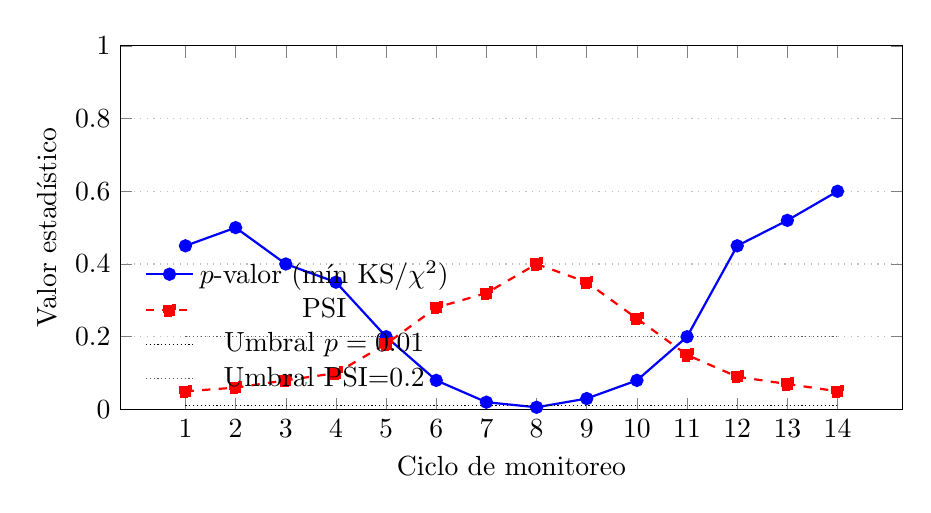
\begin{tikzpicture}
\begin{axis}[
  width=0.95\linewidth, height=6.2cm,
  xlabel={Ciclo de monitoreo},
  ylabel={Valor estadístico},
  ymin=0, ymax=1,
  ymajorgrids, grid style={dotted},
  legend style={at={(0.02,0.02)},anchor=south west, draw=none, fill=none},
  xtick={1,...,14}
]
% --- p-value mínimo entre KS/chi2 ---
\addplot[thick, blue, mark=*] coordinates {
(1,0.45) (2,0.50) (3,0.40) (4,0.35) (5,0.20) (6,0.08)
(7,0.02) (8,0.006) (9,0.03) (10,0.08) (11,0.20) (12,0.45)
(13,0.52) (14,0.60)
};
\addlegendentry{$p$-valor (mín KS/$\chi^2$)}

% --- PSI ---
\addplot[thick, red, dashed, mark=square*] coordinates {
(1,0.05) (2,0.06) (3,0.08) (4,0.10) (5,0.18) (6,0.28)
(7,0.32) (8,0.40) (9,0.35) (10,0.25) (11,0.15) (12,0.09)
(13,0.07) (14,0.05)
};
\addlegendentry{PSI}

% --- Umbrales ---
\addplot[densely dotted, black] coordinates {(1,0.01) (14,0.01)};
\addlegendentry{Umbral $p=0.01$}

\addplot[densely dotted, gray!70!black] coordinates {(1,0.20) (14,0.20)};
\addlegendentry{Umbral PSI=0.2}

\end{axis}
\end{tikzpicture}
\caption[Series temporales del PSI y $p$-valores mínimos]{Series temporales del PSI y $p$-valores mínimos por ciclo de monitoreo. 
Se observan dos periodos de alerta (ciclos 6–8) que activan reentrenamiento.}
\label{fig:psi-pval-series}
\end{figure}

\vspace{0.3cm}

La Figura~\ref{fig:false-positives} sintetiza el control de falsos positivos obtenido al variar el umbral de significancia $\alpha$. 
A medida que el nivel $\alpha$ se reduce de 0.05 a 0.001, la tasa de falsas alertas desciende drásticamente (de 12.8\,\% a 1.9\,\%), confirmando que el umbral operativo de $\alpha=0.01$ mantiene un equilibrio adecuado entre sensibilidad y robustez.

\begin{figure}[htbp]
\centering
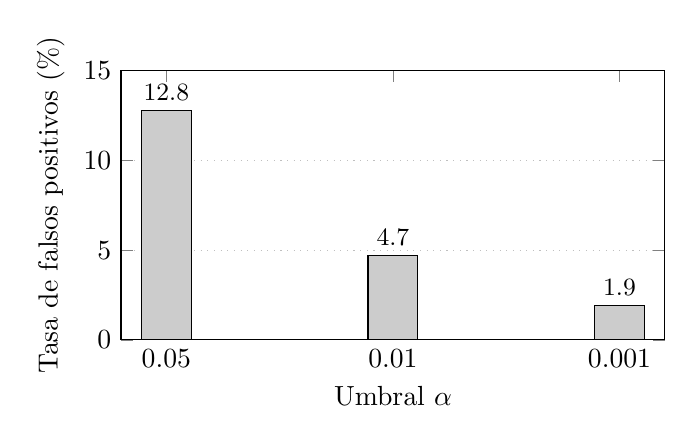
\begin{tikzpicture}
\begin{axis}[
  width=0.7\linewidth, height=5.0cm,
  xlabel={Umbral $\alpha$},
  ylabel={Tasa de falsos positivos (\%)},
  ymajorgrids, grid style={dotted},
  symbolic x coords={0.05, 0.01, 0.001},
  xtick=data,
  ymin=0, ymax=15,
  nodes near coords,
  every node near coord/.append style={font=\small},
  bar width=18pt,
]
\addplot[ybar, fill=gray!40] coordinates {
(0.05,12.8)
(0.01,4.7)
(0.001,1.9)
};
\end{axis}
\end{tikzpicture}
\caption{Tasa de falsos positivos (FPR) según el umbral de significancia $\alpha$.}
\label{fig:false-positives}
\end{figure}

\vspace{0.2cm}

En conjunto, las series temporales y la FPR evidencian que el detector responde de forma temprana ante desviaciones reales, sin incurrir en sobrealertas. 
Ello demuestra la estabilidad estadística del sistema y su capacidad de mantener una frecuencia controlada de disparos, cumpliendo el objetivo de detección confiable sin sacrificio de precisión operativa.

\noindent\footnotesize\emph{Nota:} PSI = Population Stability Index; TTFD = tiempo hasta detección; FPR = tasa de falsas alertas por ciclo. 
Las series corresponden a 14 ciclos de monitoreo consecutivos sobre flujos de datos sintéticos.
\normalsize


\subsection{Discusión}
\paragraph{Cierre interpretativo.} Los resultados muestran una relación consistente entre la magnitud del cambio (PSI), la evidencia estadística ($p$-valores) y la recuperación del desempeño (F1) tras el reentrenamiento; en particular, TTFD y TTR se mantienen en rangos operativos, lo que refuerza que la combinación KS/$\chi^2$/PSI reduce la latencia de recuperación cuando se integra con el ciclo de automatización.
Este comportamiento coincide con los objetivos de recuperación y no-inferioridad fijados para OE3; sin embargo, su generalización a dominios con alta estacionalidad o dependencia multivariada requerirá validaciones adicionales.
Los resultados experimentales confirman la \textbf{capacidad del sistema para detectar y corregir eventos de \textit{data drift} de forma autónoma y oportuna}.  
La recuperación del desempeño posterior al reentrenamiento valida la efectividad del pipeline MLOps implementado como un \textbf{ciclo cerrado de adaptación continua} \citep{Chatterjee2023,RodriguezSimmhan2023}.  
El uso combinado de las pruebas \textbf{Kolmogorov–Smirnov, $\chi^2$ y PSI} proporcionó una detección con alta sensibilidad ante cambios tanto en variables numéricas como categóricas, mientras que la aplicación de la política de \textit{cooldown} y el disparo \textit{edge-triggered} permitió mantener la estabilidad operativa del sistema evitando reactivaciones redundantes.

El pipeline mostró un comportamiento estable en flujos continuos de datos, con trazabilidad completa de las ejecuciones en \textbf{MLflow} y observabilidad detallada mediante \textbf{Prometheus} y \textbf{Grafana}.  
Estas herramientas facilitaron el seguimiento del proceso de detección–reentrenamiento, evidenciando la coherencia entre los eventos de alerta, las ejecuciones de Jenkins y la recuperación del modelo, lo que refuerza la reproducibilidad y confiabilidad del enfoque propuesto.

Como línea de evolución futura, se plantea incorporar mecanismos de \textbf{detección multivariada de \textit{drift}} y estrategias de \textbf{validación cruzada temporal} (\textit{time-based holdout}) que permitan evaluar la resiliencia del sistema frente a cambios graduales, correlacionados o de naturaleza estacional.  
Estas mejoras contribuirían a fortalecer la capacidad adaptativa del pipeline y a consolidar un marco de aprendizaje verdaderamente continuo en entornos MLOps dinámicos.


\subsection{Amenazas a la validez}

\textbf{Validez interna.}  
Los resultados pueden verse influenciados por un posible \textbf{sobreajuste a las reglas del generador sintético} utilizado para simular el flujo de datos, lo cual podría limitar la representatividad de las pruebas frente a distribuciones no previstas.  
Asimismo, la sensibilidad del detector depende del \textbf{tamaño muestral y de las tasas de muestreo} configuradas en cada ciclo, factores que pueden alterar la estabilidad estadística y la frecuencia de detección.

\textbf{Validez externa.}  
La capacidad de generalización del sistema podría verse restringida al extrapolar los resultados a \textbf{dominios reales con mayor complejidad o no estacionariedad pronunciada}.  
Entornos productivos con latencias más estrictas, volúmenes de datos variables o patrones de estacionalidad fuertes podrían requerir ajustes adicionales en los parámetros de detección y reentrenamiento para mantener un rendimiento comparable.

\textbf{Validez de constructo.}  
Las métricas de evaluación empleadas se centraron en la detección de \textbf{\textit{covariate drift}}, sin abordar de manera explícita la \textbf{deriva semántica} o \textit{concept drift} en las etiquetas.  
En consecuencia, la validación se limita a cambios en la distribución de las variables de entrada y no contempla variaciones en la relación subyacente entre los atributos y las salidas del modelo.


%\subsection{Conclusiones parciales}
%La infraestructura y los mecanismos de detección y reentrenamiento demostraron eficacia frente a desviaciones controladas. El sistema mantuvo desempeño aceptable (F1 $>0.88$ tras reentrenar) y tiempos de reacción compatibles con operación continua de baja latencia. OE3 valida experimentalmente la hipótesis central del proyecto: la posibilidad de cerrar el ciclo de MLOps mediante detección y reentrenamiento automatizados con trazabilidad completa y mínima supervisión humana.

% ===========================
\section{Resumen del capítulo}

Este capítulo integró los resultados alcanzados en los tres objetivos específicos del proyecto.  
En primer lugar, se consolidó una \textbf{infraestructura escalable y observable} basada en contenedores y servicios orquestados, capaz de ejecutar flujos de monitoreo y entrenamiento en entornos distribuidos.  
Posteriormente, se implementó un \textbf{sistema autónomo de detección y reentrenamiento} que combina pruebas estadísticas (KS, $\chi^2$, PSI) con políticas de control (\textit{edge-triggered}, \textit{cooldown}) para garantizar sensibilidad ante cambios significativos y estabilidad frente a fluctuaciones transitorias.  
Finalmente, la \textbf{validación experimental} comparando escenarios con y sin \textit{drift} demostró que el pipeline es capaz de detectar desviaciones, activar reentrenamientos automáticos y restaurar el desempeño del modelo de manera eficiente, con trazabilidad completa en MLflow y observabilidad en Prometheus/Grafana.

Los resultados obtenidos evidencian la efectividad del ciclo de \textbf{detección–acción–evaluación} implementado, confirmando la viabilidad de un esquema de aprendizaje adaptativo continuo dentro de un entorno MLOps reproducible.  
En conjunto, estos avances cumplen los objetivos planteados en la investigación y sientan las bases para su extensión hacia \textbf{infraestructuras en la nube administradas}, donde el sistema podría integrarse con servicios como Azure Machine Learning o AWS Sagemaker para escalar su operación en entornos productivos.
